%% week45rnn.tex -- Recurrent neural networks, the complete lecture
%% (Chapter 11).  Made 2026-11-07 as a stand-alone lecture, separate from the
%% week-45 Monday lecture of November 2 (which stopped at the simple RNN):
%% it merges (i) the full week-45 deck with the LSTM/GRU frames and the
%% spoken-digit demonstration (Slides/_to_delete/week45slides_v2_lstm.tex),
%% (ii) the material of doc/BookML/rnnadd.tex (the FYS5429 lectures on
%% recurrent dynamics: the state-space form, the three views of BPTT with
%% the worked two-step example, eigenmodes and transient growth, truncated
%% BPTT in practice, one-step fit against free rollout), translated to the
%% chapter's notation and placed where it belongs, and (iii) the Pause-and-
%% think frames.  All code is TensorFlow/Keras or PyTorch; the theory is
%% measured on the library layers with torch.autograd.  Figures:
%% week45rnn_*.pdf from make_week45rnn_figures.py, the TikZ schematics of the
%% book (rnnunroll, rnnlosspaths, lstmcell) and the Raschka et al. figures
%% RNN1-12 / LSTM1-10 of doc/pub/week47/ipynb/figslides/.  The companion
%% notebook week45rnn.ipynb carries all the code.
%% Book references (chapter11.tex as extended 2026-11-02; rebuild book.aux):
%% Sections 11.1-11.9 incl. 11.3.1, 11.4.1-11.4.7, 11.5.2-11.5.4, 11.6.1-11.6.2;
%% Eqs 11.1-11.13 (tasks ... oscillator), 11.18-11.21 (state space, linear
%% RNN), 11.22-11.45 (BPTT), 11.46-11.47 (weighted cost, output error),
%% 11.49-11.52 (step Jacobian, g-recursion, delta recursion, three steps),
%% 11.53-11.55 (outer products, all gradients), 11.56-11.34 (path sum),
%% 11.35 (cost of BPTT), 11.36-11.37 (discrete adjoint), Theorem 11.1 with
%% 11.38-11.39, Corollary 11.2 with 11.40, 11.41-11.44 (eigenmodes, delayed
%% copy, non-normal, contraction), 11.45 (truncated BPTT), 11.46-11.47 and
%% Proposition 11.3 (clipping), 11.48 (rollout), 11.49-11.52 (LSTM), 11.53
%% (cell path), Proposition 11.4 with 11.54-11.55, 11.56 (GRU); Figs 11.1
%% (unrolled), 11.2 (loss paths), 11.3 (gradients), 11.4 (oscillator), 11.5
%% (LSTM cell), 11.6 (frameworks); Table 11.1.
%% Build:  pdflatex week45rnn.tex  (twice)
\documentclass[10pt,aspectratio=169]{beamer}
\usetheme{red_plain}
\usepackage[T1]{fontenc}
\usepackage[utf8]{inputenc}
\usepackage{amsmath,amssymb,bm}
\usepackage{graphicx}
\usepackage{listings}
\usepackage{xcolor}
\usepackage{booktabs}
\usepackage{tikz}
\usetikzlibrary{arrows.meta,positioning}
\graphicspath{{../BookFigures/chapter11_recurrent_networks/}{../../pub/week47/ipynb/figslides/}{./ch11/}{./figslides/}{./}}

%% ---- code listings
\definecolor{codebg}{rgb}{0.97,0.97,0.97}
\lstset{language=Python,basicstyle=\ttfamily\scriptsize,backgroundcolor=\color{codebg},
  keywordstyle=\color{blue!70!black}\bfseries,commentstyle=\color{green!45!black},
  stringstyle=\color{red!60!black},showstringspaces=false,frame=single,
  framerule=0pt,xleftmargin=4pt,xrightmargin=4pt,breaklines=true,columns=fullflexible}

%% ---- the "pause and think" question frames
\newcounter{insight}
\newenvironment{insight}[1][]{%
  \stepcounter{insight}%
  \begin{frame}{Pause and think \arabic{insight}: #1}%
  \setbeamercolor{block title}{bg=structure.fg,fg=white}%
  \setbeamercolor{block body}{bg=structure.fg!8}%
  \small
}{\end{frame}}
\newcommand{\question}[1]{\begin{block}{Question}#1\end{block}}
\newcommand{\answer}[1]{\pause\begin{block}{Answer}#1\end{block}}

\setbeamertemplate{footline}[frame number]
\setbeamerfont{block title}{size=\small}
\setbeamertemplate{blocks}[rounded][shadow=false]
\setbeamercovered{invisible}

\title{Recurrent Neural Networks}
\subtitle{The complete lecture: sequences and the hidden state, where the
  recurrence comes from, backpropagation through time in three views, why
  long sequences are hard, gated cells -- all of it in TensorFlow/Keras and
  PyTorch\\[3pt]
  \small With pauses for questions}
\author{Morten Hjorth-Jensen}
\institute{Department of Physics and Center for Computing in Science Education,\\
  University of Oslo, Norway}
\date{}

\begin{document}

\begin{frame}
\titlepage
\end{frame}

\begin{frame}{Plan for this lecture}
\small
\textbf{Chapter 11 in one sitting, with every code example in TensorFlow/Keras
or PyTorch:}
\begin{enumerate}
  \item \textbf{From feed-forward to recurrent networks}: what we give up,
        what a sequence model is asked to do, the hidden state.
  \item \textbf{The architecture}: the simple RNN, folded and unrolled; the
        RNN as a dynamical system.
  \item \textbf{Where the recurrence comes from}: a damped oscillator, Euler's
        method as a recurrence, the state-space form, and why the integrator
        matters.
  \item \textbf{The layers in Keras and PyTorch}: what \texttt{SimpleRNN} and
        \texttt{nn.RNN} compute, line by line.
  \item \textbf{Backpropagation through time, three ways}: the recursion of
        the chapter, the pre-activation error and the outer products, the
        path sum; a worked example checked with autograd; the discrete
        adjoint; what \texttt{loss.backward()} does.
  \item \textbf{Why long sequences are hard}: the Jacobian product measured;
        eigenmodes, saturation and transient growth; truncated BPTT in
        practice; clipping; a network that learns the rule of an oscillator,
        and what a free rollout reveals.
  \item \textbf{Long short-term memory and the GRU}: gates, the cell state, by
        how much it helps.
  \item \textbf{Four applications}: a sine wave, MNIST row by row, spoken
        digits, and the adding problem.
\end{enumerate}
\textbf{Reading:} Chapter 11 (all of it); Goodfellow et al.\ Chapter 10;
Raschka et al.\ Chapter 15; Pascanu, Mikolov and Bengio (ICML 2013).  The
code is in \texttt{week45rnn.ipynb}.
\end{frame}

%% =====================================================================
\section{From feed-forward to recurrent networks}
\begin{frame}{What we have assumed so far, 1: independent samples}
Almost everything since week 35 -- the bias-variance decomposition, the
bootstrap, cross-validation, the statistical toolbox of Chapter 2 -- leans
on the training examples being \emph{independent and identically
distributed}.

\medskip
For a sequence this is simply false.  The value of a detector trace at one
sample is strongly informative about the next; that is the entire content
of the data.

\medskip
\begin{block}{The consequence}
A model that treats the samples as independent has thrown the signal away
before it starts.
\end{block}
\end{frame}

\begin{frame}{What we have assumed so far, 2: a fixed input size}
A feed-forward network has a fixed input dimension.  A convolutional
network (week 44) has one too, up to the pooling that precedes its dense
layers.

\medskip
Sequences come in different lengths -- a measurement that ran for ten
seconds and one that ran for an hour, a spoken word of $0.3$ s and one of
$0.6$ s -- and we would like \emph{one} model to handle all of them.
\end{frame}

\begin{frame}{The move of this chapter}
\begin{block}{Week 44}
We restricted the dense layer so that it respects the \emph{spatial}
structure of an image, and obtained \emph{convolution}.
\end{block}
\begin{block}{Today}
We make the same kind of restriction for data with a \emph{temporal}
structure, and obtain \emph{recurrence}: process one element at a time and
carry a state forward, so that the same parameters serve a sequence of any
length.
\end{block}
\end{frame}

\begin{frame}{Sequences in the physical sciences}
Ordered, correlated data are the norm rather than the exception:
\begin{itemize}
  \item detector read-out streams and waveform traces;
  \item climate and seismic records;
  \item molecular-dynamics trajectories and spectroscopy scans;
  \item state estimation in control and feedback;
  \item the solutions of differential equations, which are time series by
        construction;
  \item sound -- which we will classify today.
\end{itemize}
\medskip
Sequential need not mean temporal (text, genomes), but our examples are
time series.  We write $x_{1:T}=(\bm{x}_1,\dots,\bm{x}_T)$.
\end{frame}

\begin{frame}{Three tasks, Eq.~(11.1)}
\begin{columns}[T]
\begin{column}{0.5\textwidth}
\[
  p(x_{1:T}),\qquad p(y_{1:T}\mid x_{1:T}),\qquad p(y\mid x_{1:T}).
\]
\begin{itemize}
  \item modelling the sequence itself;
  \item mapping a sequence to a sequence: filtering, forecasting
        (\emph{many-to-many});
  \item mapping a sequence to one label: classification, regime detection
        (\emph{many-to-one}).
\end{itemize}
\medskip
Today: the oscillator and the sine wave are many-to-many; MNIST, the spoken
digits and the adding problem are many-to-one.
\end{column}
\begin{column}{0.48\textwidth}
\begin{center}
\includegraphics[width=0.8\textwidth]{RNN5}\\
\scriptsize Figures in this part from Raschka and Mirjalili, \emph{Python
Machine Learning}.
\end{center}
\end{column}
\end{columns}
\end{frame}

\begin{frame}{What is a recurrent neural network?}
\begin{columns}[T]
\begin{column}{0.46\textwidth}
In a feed-forward network the information flows in one direction only,
from the input to the output.

\medskip
A recurrent network also has connections pointing \emph{backward}: the
hidden layer is connected to \emph{itself}.  The hidden state at step $t$
receives two inputs -- the data $\bm{x}^{(t)}$ and its own value
$\bm{h}^{(t-1)}$ from the previous step.

\medskip
\begin{block}{What this buys}
A \emph{memory} across time steps, and the same layer for the first element
of a sequence and the thousandth.
\end{block}
\end{column}
\begin{column}{0.52\textwidth}
\begin{center}
\includegraphics[width=\textwidth]{RNN1}
\end{center}
\end{column}
\end{columns}
\end{frame}

\begin{frame}{Fold and unfold: two drawings of the same computation}
\begin{center}
\includegraphics[width=0.6\textwidth]{RNN2}
\end{center}
\begin{columns}[T]
\begin{column}{0.48\textwidth}
\begin{block}{Folded (left)}
A single layer with an arrow leaving it and returning to itself.  This is
how the network is \emph{stored}: one copy of the weights.
\end{block}
\end{column}
\begin{column}{0.48\textwidth}
\begin{block}{Unrolled (right)}
The same layer drawn once per time step.  This is how the network is
\emph{executed} -- and, as we will see, how it is \emph{differentiated}.
\end{block}
\end{column}
\end{columns}
\end{frame}

\begin{frame}{The hidden state: a latent state-space model}
The chain rule of probability factorises the first task exactly, Eq.~(11.2),
\[
  p(x_{1:T}) = \prod_{t=1}^{T} p\!\left(\bm{x}_t \mid x_{1:t-1}\right),
\]
exact and useless as it stands: the conditioning set grows without bound.
What makes it tractable is the assumption that everything relevant in
$x_{1:t-1}$ can be summarised in a finite-dimensional \emph{state}
$\bm{h}_t$, updated recursively, Eq.~(11.3):
\[
  \boxed{\;\bm{h}_t = f_\theta\!\left(\bm{h}_{t-1},\bm{x}_t\right),\qquad
  \hat{\bm{y}}_t = g_\theta\!\left(\bm{h}_t\right).\;}
\]
\begin{block}{This should look familiar}
Equation~(11.3) is the structure of a \emph{Markovian dynamical system}.
The Kalman filter is the case where $f_\theta$ is linear and the noise
Gaussian.  A recurrent neural network is the case where $f_\theta$ and
$g_\theta$ are neural networks -- the update map is \emph{learned}.
\end{block}
\end{frame}

%% =====================================================================
\section{The architecture}
\begin{frame}{The simple RNN, Eq.~(11.4)}
\begin{columns}[T]
\begin{column}{0.5\textwidth}
One affine map and one activation per step:
\[
\begin{aligned}
  \bm{a}^{(t)} &= \bm{U}\bm{x}^{(t)} + \bm{W}\bm{h}^{(t-1)} + \bm{b},\\
  \bm{h}^{(t)} &= \sigma_h\!\left(\bm{a}^{(t)}\right),\\
  \bm{o}^{(t)} &= \bm{V}\bm{h}^{(t)} + \bm{c},\\
  \hat{\bm{y}}^{(t)} &= \sigma_y\!\left(\bm{o}^{(t)}\right),
\end{aligned}
\]
$\bm{U}\in\mathbb{R}^{n_h\times n_x}$ maps the input into the state,
$\bm{W}\in\mathbb{R}^{n_h\times n_h}$ the state to itself,
$\bm{V}\in\mathbb{R}^{n_y\times n_h}$ reads the state out; $\bm{h}^{(0)}=\bm{0}$.

\medskip
$\sigma_h$ is almost always $\tanh$ (Part 5 says why); $\sigma_y$ is the
identity for regression, the softmax for classification.
\end{column}
\begin{column}{0.48\textwidth}
\begin{center}
\includegraphics[width=\textwidth]{RNN8}\\
\scriptsize Raschka's notation: $\bm{U}=\bm{W}_{hx}$, $\bm{W}=\bm{W}_{hh}$,
$\bm{V}=\bm{W}_{yh}$.
\end{center}
\end{column}
\end{columns}
\end{frame}

\begin{frame}{The same arrays at every step (Figure 11.1)}
\begin{center}
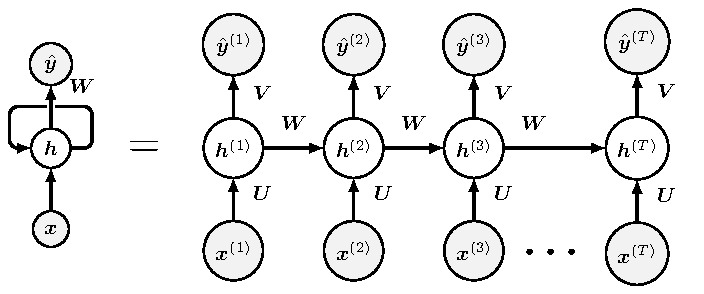
\includegraphics[width=0.55\textwidth]{rnnunroll}
\end{center}
\begin{block}{The parameters do not depend on $t$}
Parameter sharing along the time axis, exactly as convolution shares
parameters along the spatial axes (week 44): the parameter count is
independent of the sequence length, and the model is equivariant to a shift
in time.
\end{block}
\end{frame}

\begin{frame}{Two more properties of Eq.~(11.4)}
\begin{block}{The state is a bottleneck}
Everything the network will ever know about $x_{1:t}$ when it predicts
$\hat{\bm{y}}^{(t+1)}$ must fit in the $n_h$ numbers of $\bm{h}^{(t)}$.
\end{block}
\begin{block}{The cost accumulates over the sequence, Eq.~(11.5)}
\[
  \mathcal{L}=\frac1T\sum_{t=1}^{T}L^{(t)},\qquad
  L^{(t)}=\tfrac12\|\hat{\bm{y}}^{(t)}-\bm{y}^{(t)}\|^2
\]
for regression, the cross entropy for classification.  In the
sequence-to-label case only $L^{(T)}$ is non-zero -- the hardest case of
all, as Part 5 will show.
\end{block}
\end{frame}

\begin{insight}[count the parameters]
\question{How many parameters has the simple RNN of Eq.~(11.4) with
$n_x=1$, $n_h=24$, $n_y=1$ -- the network we train on the oscillator in
Part 5?  How many would a dense network need if a sequence of length
$T=40$ were flattened into one input vector, with the same $24$ hidden
nodes?  And what happens to each count when $T$ becomes $400$?}
\answer{$\bm{U}$: $24\times1$, $\bm{W}$: $24\times24=576$, $\bm{b}$: $24$,
$\bm{V}$: $1\times24$, $\bm{c}$: $1$ -- in total
$n_h(n_x+n_h+1)+n_y(n_h+1)=24\cdot26+25=649$, and $T$ appears nowhere.
The flattened dense network has $40\times24+24+24+1=1009$ parameters at
$T=40$ and $9649$ at $T=400$ -- and must be \emph{retrained} for every new
$T$.  The recurrent network has $649$ either way.  (Keras will print
exactly $649$ for this model; PyTorch prints $673$ -- Part 3 explains
the difference.)}
\end{insight}

\begin{frame}{Stacking: a multilayer RNN}
\begin{columns}[T]
\begin{column}{0.42\textwidth}
The hidden state of one recurrent layer can be the input sequence of the
next.  Each layer has its own $\bm{U},\bm{W},\bm{b}$ and is unrolled along
the same time axis, so the unrolled graph becomes a grid: depth in layers
downwards, depth in time sideways.

\medskip
In the libraries: \texttt{num\_layers=2} in \texttt{nn.RNN}, or two
\texttt{SimpleRNN} layers with \texttt{return\_sequences=True} in Keras.
\end{column}
\begin{column}{0.56\textwidth}
\begin{center}
\includegraphics[width=\textwidth]{RNN3}
\end{center}
\end{column}
\end{columns}
\end{frame}

\begin{frame}{The RNN as a discrete-time dynamical system (Section 11.2.1)}
Set the input to zero.  Equation~(11.4) becomes an autonomous map,
Eq.~(11.6),
\[
  \bm{h}^{(t)} = F\!\left(\bm{h}^{(t-1)}\right)
  := \sigma_h\!\left(\bm{W}\bm{h}^{(t-1)}+\bm{b}\right).
\]
Fixed points satisfy $\bm{h}^\star=F(\bm{h}^\star)$; their stability is
decided by the Jacobian, Eq.~(11.7),
\[
  \bm{J}=\left.\frac{\partial F}{\partial\bm{h}}\right|_{\bm{h}^\star}
  =\operatorname{diag}\!\left(\sigma_h'(\bm{a}^\star)\right)\bm{W},
\]
attracting if the spectral radius $\rho(\bm{J})<1$, repelling if
$\rho(\bm{J})>1$.  In two dimensions the map can have limit cycles, in three
or more it can be chaotic.
\end{frame}

\begin{frame}{Why this matters, twice}
\begin{block}{What a recurrent network can represent}
Oscillations, decay to a point attractor, chaotic wandering.
\end{block}
\begin{block}{What it does with information}
Strongly contracting dynamics forget the initial condition quickly and
cannot carry information far; expanding dynamics are unstable.
\end{block}
\medskip
Equation~(11.7) is also exactly the quantity that will control the gradient
in Part 5: the stability of the forward dynamics and the survival of the
backward gradient are the \emph{same question}.
\end{frame}

\begin{frame}{The one-dimensional map, and an untrained \texttt{nn.RNN} (\texttt{week45rnn\_dynamics.pdf})}
\begin{center}
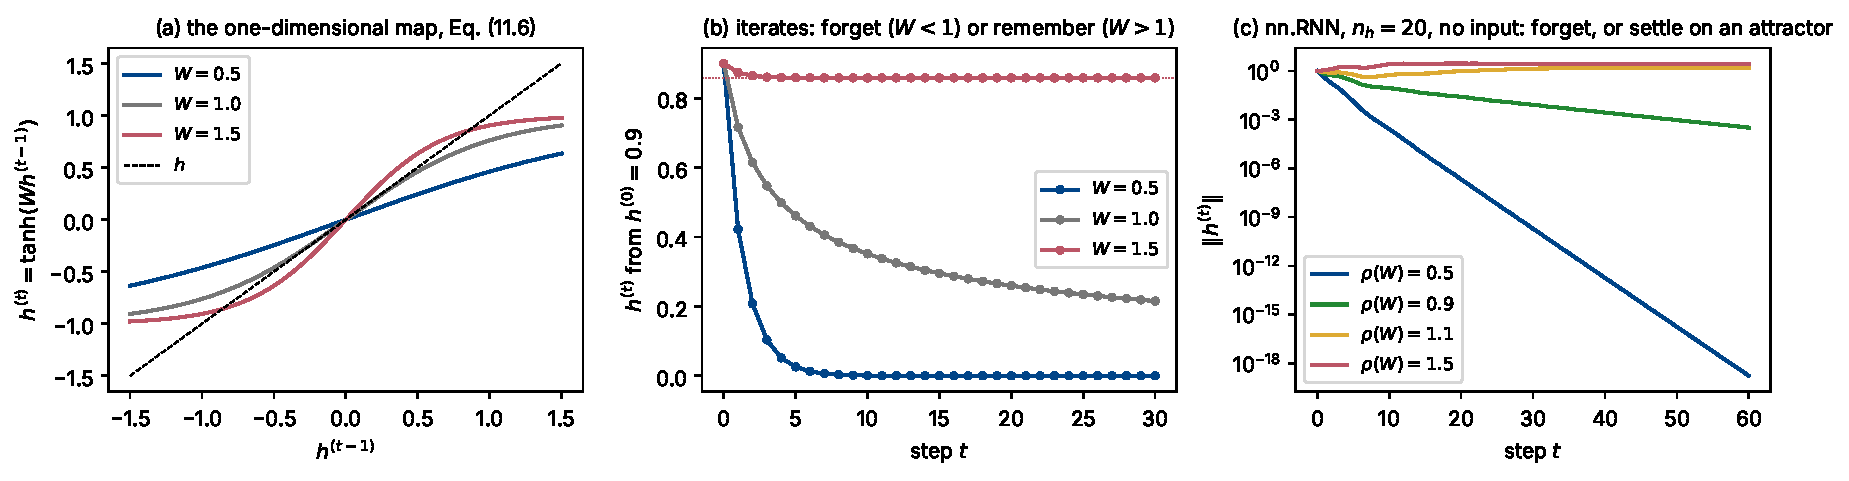
\includegraphics[width=\textwidth]{week45rnn_dynamics}
\end{center}
\small
(a) $h\mapsto\tanh(Wh)$ against the diagonal: for $W<1$ the only fixed point
is $0$, for $W>1$ two new ones appear.  (b) Iterates from $h^{(0)}=0.9$: at
$W=0.5$ the state is gone after ten steps, at $W=1.5$ it sits on
$h^\star=\pm0.8586$ for ever.  (c) A PyTorch \texttt{nn.RNN} with $n_h=20$,
zero input, $\bm{W}$ scaled to a given spectral radius: at $\rho(\bm{W})=0.5$
the norm of the state falls by nineteen orders of magnitude in sixty steps;
at $\rho>1$ it settles on an attractor of order one.
\end{frame}

\begin{insight}[forget or remember]
\question{For the one-dimensional map $h^{(t)}=\tanh(Wh^{(t-1)})$ (no
bias): show that $h^\star=0$ is always a fixed point, decide when it is
stable, and say what happens at $W=1$.  What does a network with
$|W|<1$ do with the information in $h^{(0)}$?}
\answer{$\tanh(0)=0$, so $0$ is a fixed point for every $W$.  Its Jacobian
is $J=\tanh'(0)\,W=W$: stable for $|W|<1$, unstable for $|W|>1$.  At $W=1$
a \emph{pitchfork bifurcation} produces two new stable fixed points
$\pm h^\star$ with $h^\star=\tanh(Wh^\star)$ -- $0.66$ at $W=1.2$, $0.86$ at
$W=1.5$, $0.96$ at $W=2$.  With $|W|<1$ every initial condition is driven
to $0$ geometrically, $|h^{(t)}|\le|W|^t|h^{(0)}|$: the network
\emph{forgets} its input at the rate $|W|^t$.  In Part 5 this very number
reappears as the size of the gradient that reaches step $0$ from step $t$.}
\end{insight}

%% =====================================================================
\section{Where the recurrence comes from}
\begin{frame}{A differential equation (Section 11.3)}
The recurrence of Eq.~(11.4) can look arbitrary.  It is not.  Newton's
equation for a damped harmonic oscillator, scaled to dimensionless time,
Eq.~(11.8):
\[
  \frac{\mathrm{d}^2x}{\mathrm{d}t^2}+\eta\frac{\mathrm{d}x}{\mathrm{d}t}+x(t)=F(t),
\]
with $\eta$ the damping and $F$ an external force.  As always we rewrite it
as two coupled first-order equations, Eq.~(11.9),
\[
  v=\frac{\mathrm{d}x}{\mathrm{d}t},\qquad
  \frac{\mathrm{d}v}{\mathrm{d}t}=F(t)-\eta v(t)-x(t),
\]
and integrate from $(x_0,v_0)$ -- by hand for $F=0$, by Runge-Kutta in
general.
\end{frame}

\begin{frame}{Discretise, and the recurrence appears}
Forward Euler for the velocity gives step $i+1$ from step $i$, Eq.~(11.10):
\[
  v_{i+1}=v_i+\Delta t\left(F_i-\eta v_i-x_i\right)=:h_i\!\left(x_i,v_i,F_i\right),
\]
a function of the \emph{current state} and the \emph{current input}.  But
$v_i$ was itself produced by the same rule one step earlier, Eq.~(11.11),
so substituting, Eq.~(11.12), and renaming, Eq.~(11.13),
\[
  v_{i+1}=h_i\!\left(x_i,\,h_{i-1},\,F_i\right)
  \qquad\Longrightarrow\qquad
  \bm{h}_i=h\!\left(\bm{x}_i,\bm{h}_{i-1}\right),
\]
which is Eq.~(11.3) exactly.
\end{frame}

\begin{frame}{Position alone is not a state (Section 11.3.1)}
\begin{block}{Two oscillators through the same point}
Two oscillators pass through the same position $x$ at the same time, one
moving left and the other right.  Their next positions differ even if the
force is identical.  \textbf{Position alone is an incomplete description};
position and velocity together are a \emph{state}: given $(x_i,v_i)$ and
the input $F_i$, the next $(x_{i+1},v_{i+1})$ is determined.
\end{block}
\begin{block}{What this says about the hidden state}
The hidden state $\bm{h}^{(t)}$ of a recurrent network has to play this role
for whatever process generated the data: it must carry \emph{everything
about the past that the future depends on}.  If the data were produced by a
second-order equation and the network is only given $x$, the network has to
\emph{reconstruct} the velocity inside $\bm{h}^{(t)}$ from consecutive
inputs -- which is what the oscillator experiment later in the lecture asks
it to do.
\end{block}
\end{frame}

\begin{frame}{The state-space form, Eqs.~(11.14)--(11.17)}
Euler for \emph{both} components, with $\bm{s}_i=(x_i,v_i)^{\mathsf{T}}$:
\[
  x_{i+1}=x_i+\Delta t\,v_i,\qquad
  v_{i+1}=\underbrace{(1-\eta\Delta t)}_{\text{recurrent weight}}v_i
         +\underbrace{\Delta t}_{\text{force weight}}F_i
         -\underbrace{\Delta t}_{\text{position coefficient}}x_i,
\]
\[
  \bm{s}_{i+1}=\bm{A}\bm{s}_i+\bm{B}F_i,\qquad
  \bm{A}=\begin{pmatrix}1&\Delta t\\-\Delta t&1-\eta\Delta t\end{pmatrix},\quad
  \bm{B}=\begin{pmatrix}0\\ \Delta t\end{pmatrix}.
\]
Unrolled, Eq.~(11.16):
$\bm{s}_n=\bm{A}^n\bm{s}_0+\sum_{i=0}^{n-1}\bm{A}^{\,n-1-i}\bm{B}F_i$ -- an
input $F_i$ reaches $\bm{s}_n$ through $n-1-i$ applications of $\bm{A}$.
\begin{block}{This \emph{is} a linear recurrent network, Eq.~(11.17)}
Set $\sigma_h=$ identity, $\bm{W}=\bm{A}$, $\bm{U}=\bm{B}$, $\bm{V}=(1,0)$,
$\bm{b}=\bm{c}=0$: Eq.~(11.4) with $\bm{h}^{(t)}=\bm{s}_t$ and
$\bm{x}^{(t)}=F_t$ reproduces forward Euler exactly.  The simple RNN is the
same object with a non-linearity and \emph{learned} coefficients.  With
$\Delta t=0.05$, $\eta=0.2$: $\bm{A}=\bigl(\begin{smallmatrix}1&0.05\\-0.05&0.99\end{smallmatrix}\bigr)$,
eigenvalues $0.995\pm0.0498\,i$, modulus $0.9962$.
\end{block}
\end{frame}

\begin{frame}{The integrator itself can amplify errors (why RK4 makes the data)}
\begin{columns}[T]
\begin{column}{0.5\textwidth}
\begin{block}{Undamped, unforced: the exact motion is bounded}
Forward Euler's matrix has eigenvalues $1\pm i\Delta t$, modulus
$\sqrt{1+\Delta t^2}=1.00125$ at $\Delta t=0.05$: the amplitude \emph{grows}
by a factor $e\approx2.7$ over the $800$ steps to $t=40$.
\end{block}
\begin{block}{Damped, $\eta=0.2$}
Euler decays by $0.9962$ per step where the exact solution decays by
$e^{-\eta\Delta t/2}=0.9950$: by $t=40$ the Euler amplitude is $2.7$ times
the true one.
\end{block}
\end{column}
\begin{column}{0.48\textwidth}
\begin{block}{Two lessons}
\begin{itemize}
  \item A network that learns the Euler update \emph{perfectly} reproduces
        this artificial growth.  The training data of this lecture are
        therefore generated by RK4, and a rollout is always compared with a
        trusted reference, so that an error in the learned dynamics can be
        told from an error already in the integrator.
  \item The modulus of the eigenvalues of the one-step map decides whether
        a perturbation grows or decays.  Keep this in mind: it is exactly the
        quantity that will govern the \emph{gradients} in Section 11.5.
\end{itemize}
\end{block}
\end{column}
\end{columns}
\end{frame}


\begin{frame}{A recurrent network is a learned, non-linear time-stepper}
\begin{block}{The correspondence}
\begin{itemize}
  \item the hidden state plays the role of the integrator's internal state;
  \item $\bm{W}$ plays the role of $1-\eta\Delta t$;
  \item the training data supply what the differential equation would
        otherwise have to tell us.
\end{itemize}
\end{block}
\medskip
The output $\hat{y}_i$ is compared with a target through a cost -- the
target being a measurement, or the solution of the equation.
\end{frame}

\begin{frame}{The data for today's experiment (\texttt{week45rnn\_oscillator\_data.pdf})}
\begin{center}
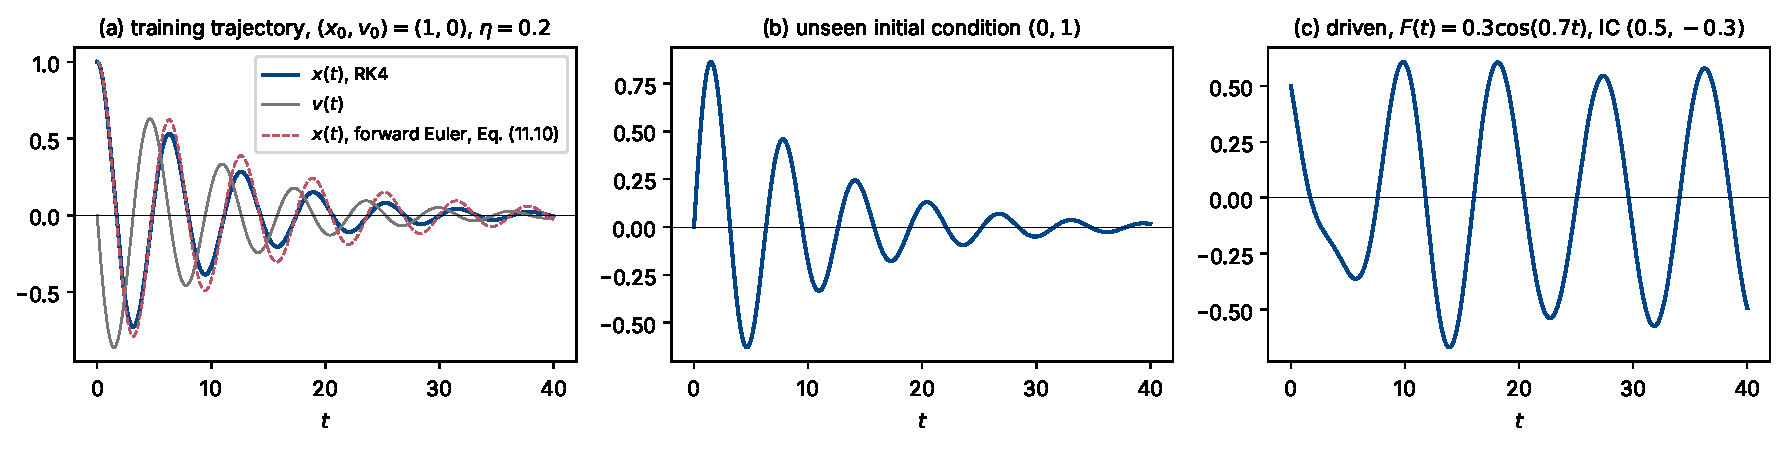
\includegraphics[width=\textwidth]{week45rnn_oscillator_data}
\end{center}
\small
Fourth-order Runge-Kutta with $\eta=0.2$ on $t\in[0,40]$, $800$ points.
Forward Euler at the same $\Delta t=0.05$ (dashed) is visibly off by the
second period -- an error of $0.1$ -- a first hint of what a \emph{learned}
stepper can improve on.  In Part 5 the network sees only the blue curve of
(a); (b) and (c) are the tests.
\end{frame}

\begin{frame}{Compare week 42: two ways to solve a differential equation with a network}
\begin{columns}[T]
\begin{column}{0.48\textwidth}
\begin{block}{Chapter 9 (week 42)}
The equation was \emph{known} and supplied the cost through its residual;
no data were needed; the network learned a function of continuous time.
\end{block}
\end{column}
\begin{column}{0.48\textwidth}
\begin{block}{Chapter 11 (today)}
The equation is \emph{unknown} and the data supply the cost; the network
learns a discrete update rule.
\end{block}
\end{column}
\end{columns}
\medskip
The first is for known physics and absent data, the second for present data
and unknown physics.
\end{frame}

%% =====================================================================
\section{The layers in Keras and PyTorch}
\begin{frame}{Two libraries, one layer}
\begin{center}
\footnotesize
\begin{tabular}{lll}
\toprule
Equation & TensorFlow/Keras & PyTorch\\
\midrule
simple RNN, Eq.~(11.4) & \texttt{layers.SimpleRNN(units)} & \texttt{nn.RNN(input\_size, hidden\_size)}\\
LSTM, Eqs.~(11.49)--(11.52) & \texttt{layers.LSTM(units)} & \texttt{nn.LSTM(input\_size, hidden\_size)}\\
GRU, Eq.~(11.56) & \texttt{layers.GRU(units)} & \texttt{nn.GRU(input\_size, hidden\_size)}\\
read-out $\bm{V}\bm{h}+\bm{c}$ & \texttt{layers.Dense(n\_y)} & \texttt{nn.Linear(hidden\_size, n\_y)}\\
clipping, Eq.~(11.46) & \texttt{Adam(lr, clipnorm=1.0)} & \texttt{nn.utils.clip\_grad\_norm\_(params, 1.0)}\\
BPTT & inside \texttt{model.fit} & \texttt{loss.backward()}\\
\bottomrule
\end{tabular}
\end{center}
\begin{block}{The one convention to remember: the data layout}
Both libraries want a 3-tensor of shape \texttt{(samples, timesteps,
features)} $=(N,T,n_x)$: $N$ sequences, each $T$ steps of $n_x$ numbers.
In PyTorch this needs \texttt{batch\_first=True} (the default is
$(T,N,n_x)$).  A single time series is \emph{cut into windows} to make the
first axis.
\end{block}
\end{frame}

\begin{frame}[fragile]{Keras: a minimal recurrent model}
\begin{lstlisting}
from tensorflow import keras
from tensorflow.keras import layers

model = keras.Sequential([
    keras.Input(shape=(None, 1)),               # (T, n_x): T may vary, one feature per step
    layers.SimpleRNN(24, return_sequences=True), # Eq. (11.4): h_t for every t, n_h = 24
    layers.Dense(1),                             # V h_t + c, applied at every step
])
model.compile(optimizer=keras.optimizers.Adam(5e-3, clipnorm=1.0), loss="mse")
model.summary()                                  # 24*(1+24+1) + 25 = 649 parameters
history = model.fit(X_train, Y_train, epochs=300, batch_size=4, verbose=0)
\end{lstlisting}
\small
\texttt{X\_train} has shape $(N,T,1)$ and \texttt{Y\_train} the shape
$(N,T,1)$ of the targets -- here one target per step, the
sequence-to-sequence case.  Six lines; the next frame reads them one by one.
\end{frame}

\begin{frame}{Keras: what each line does}
\small
\begin{description}
  \item[\texttt{Input(shape=(None, 1))}] the shape of \emph{one} sample
        without the batch axis: $T$ steps (\texttt{None} = any length) of
        $n_x=1$ features.
  \item[\texttt{SimpleRNN(24)}] one recurrent layer with $n_h=24$: $\bm{U}$
        ($1\times24$, stored transposed as \texttt{kernel}), $\bm{W}$
        ($24\times24$, \texttt{recurrent\_kernel}), $\bm{b}$ (\texttt{bias});
        $\tanh$ by default; $\bm{h}^{(0)}=\bm{0}$.
  \item[\texttt{return\_sequences=True}] output all of $\bm{h}^{(1)},\dots,\bm{h}^{(T)}$,
        shape $(N,T,24)$.  With \texttt{False} (the default) only
        $\bm{h}^{(T)}$, shape $(N,24)$ -- the sequence-to-label case.
  \item[\texttt{Dense(1)}] $\bm{V}\bm{h}+\bm{c}$.  Applied to a 3-tensor it
        acts on the last axis, i.e.\ at every time step with the same
        $\bm{V},\bm{c}$.
  \item[\texttt{compile(...)}] the optimiser (Adam, week 38) and the cost;
        \texttt{clipnorm=1.0} is gradient clipping, Eq.~(11.46), on the whole
        gradient vector.
  \item[\texttt{fit(...)}] forward pass, backpropagation through time and the
        update, \texttt{epochs} times over all windows in mini-batches of
        \texttt{batch\_size} windows.
\end{description}
\end{frame}

\begin{frame}{Keras: the knobs you will actually use}
\small
\begin{itemize}
  \item \texttt{SimpleRNN} $\to$ \texttt{LSTM} $\to$ \texttt{GRU}: change
        one word; the shapes of input and output are the same.
  \item \texttt{return\_sequences=True} on every layer but the last to
        \emph{stack} recurrent layers; \texttt{return\_state=True} to also
        get the final state (for the LSTM both $\bm{h}^{(T)}$ and
        $\bm{c}^{(T)}$).
  \item \texttt{Input(shape=(T, n\_x))} with a fixed $T$ when all windows
        have the same length (faster); \texttt{None} when they do not.
  \item Variable-length sequences in one batch: pad, and put a
        \texttt{layers.Masking(mask\_value=0.0)} first so that padded steps
        are skipped.
  \item Classification from the last state: \texttt{Dense(n\_classes)}
        with \texttt{SparseCategoricalCrossentropy(from\_logits=True)} --
        the softmax and the cross entropy of week 41 in one object.
  \item \texttt{LSTM(..., unit\_forget\_bias=True)} is the default: the
        forget gate starts at $\sigma(1)\approx0.73$ (Part 6).
\end{itemize}
\end{frame}

\begin{frame}[fragile]{PyTorch: the same model}
\begin{lstlisting}
import torch, torch.nn as nn

class Forecaster(nn.Module):
    def __init__(self, n_h=24):
        super().__init__()
        self.rnn = nn.RNN(input_size=1, hidden_size=n_h, batch_first=True)  # Eq. (11.4), tanh
        self.fc = nn.Linear(n_h, 1)                                         # V h_t + c

    def forward(self, x):                   # x: (N, T, 1)
        H, h_T = self.rnn(x)                # H: (N, T, n_h) = every h_t;  h_T: (1, N, n_h)
        return self.fc(H)                   # (N, T, 1): one prediction per step

model = Forecaster()
print(sum(p.numel() for p in model.parameters()))   # 673 (two bias vectors, see below)
\end{lstlisting}
\small
PyTorch separates the \emph{definition} of the network (a class with a
\texttt{forward}) from its \emph{training} (a loop you write).  Keras hides
the loop in \texttt{fit}; PyTorch shows it -- which is why we use it when we
want to see the gradients.
\end{frame}

\begin{frame}{PyTorch: what each line does}
\small
\begin{description}
  \item[\texttt{nn.RNN(input\_size, hidden\_size, batch\_first=True)}]
        Eq.~(11.4) with $\tanh$ (\texttt{nonlinearity="relu"} is the other
        option).  \texttt{batch\_first=True} makes the input $(N,T,n_x)$.
        \texttt{num\_layers=2} stacks two layers.
  \item[\texttt{self.rnn(x)} returns a pair] \texttt{H} of shape $(N,T,n_h)$
        with all hidden states, and \texttt{h\_T} of shape
        $(\texttt{num\_layers},N,n_h)$ with the last one.  You choose: all of
        \texttt{H} for sequence-to-sequence, \texttt{H[:, -1, :]} for
        sequence-to-label.
  \item[the parameters] \texttt{weight\_ih\_l0} is $\bm{U}$ ($n_h\times n_x$),
        \texttt{weight\_hh\_l0} is $\bm{W}$, and there are \emph{two} biases
        \texttt{bias\_ih\_l0} and \texttt{bias\_hh\_l0} whose sum is our
        $\bm{b}$ -- hence $673=649+24$.
  \item[\texttt{nn.Linear(n\_h, 1)}] $\bm{V}\bm{h}+\bm{c}$ on the last axis,
        exactly like Keras's \texttt{Dense}.
  \item[\texttt{nn.LSTM}, \texttt{nn.GRU}] same calls, same shapes;
        \texttt{nn.LSTM} returns \texttt{(H, (h\_T, c\_T))}, with the cell
        state as well.
\end{description}
\end{frame}

\begin{frame}[fragile]{PyTorch: the training loop, line by line}
\begin{lstlisting}
opt = torch.optim.Adam(model.parameters(), lr=5e-3)
lossfn = nn.MSELoss()
for epoch in range(300):
    for idx in torch.randperm(len(X_train)).split(4):        # shuffle windows, batches of 4
        opt.zero_grad()                                        # forget last batch's gradients
        loss = lossfn(model(X_train[idx]), Y_train[idx])      # forward pass, Eq. (11.5)
        loss.backward()                                        # BPTT, Eqs. (11.20)-(11.22)
        gnorm = nn.utils.clip_grad_norm_(model.parameters(), 1.0)   # Eq. (11.46); returns ||g||
        opt.step()                                             # Adam update, week 38
\end{lstlisting}
\small
\begin{itemize}
  \item \texttt{randperm(...).split(4)}: the \emph{windows} are shuffled,
        the time order inside each window is not.
  \item \texttt{zero\_grad()}: PyTorch \emph{accumulates} gradients into
        \texttt{.grad}, so each batch starts by clearing them.
  \item \texttt{loss.backward()}: automatic differentiation through the
        unrolled graph -- Part 4 says what it computes.
  \item \texttt{clip\_grad\_norm\_} rescales the whole gradient in place if
        its norm exceeds $1$ and returns the norm \emph{before} clipping --
        which is how we will look at it.
\end{itemize}
\end{frame}

\begin{frame}[fragile]{Counting parameters in both libraries}
\begin{lstlisting}
 cell        Keras   PyTorch   formula n_h(n_x+n_h+1)      n_x=1, n_h=24
 simple RNN     624       648       624
 LSTM          2496      2592      2496   (4 gates: four times the simple RNN)
 GRU           1944      1944      1872   (3 gates: three times)
\end{lstlisting}
\small
\begin{itemize}
  \item Keras's \texttt{SimpleRNN} and \texttt{LSTM} print exactly
        Eq.~(11.4) and $4\times$Eq.~(11.4).  Use this as a check: if the LSTM
        is not four times the simple RNN, something is wrong.
  \item PyTorch is larger by $n_h$ per gate: the second bias vector.  The
        model is the same, only the parameterisation is redundant.
  \item Keras's \texttt{GRU} uses \texttt{reset\_after=True} (the cuDNN
        convention) which also carries two biases -- hence $1944$ in both.
\end{itemize}
\end{frame}

\begin{frame}[fragile]{Same weights, same outputs: the conventions (Section 11.8.3)}
\begin{lstlisting}
rnn = nn.RNN(n_x, n_h, batch_first=True)                 # PyTorch, random weights
U = rnn.weight_ih_l0.detach().numpy()                     # (n_h, n_x)
W = rnn.weight_hh_l0.detach().numpy()                     # (n_h, n_h)
b = (rnn.bias_ih_l0 + rnn.bias_hh_l0).detach().numpy()    # one bias in Eq. (11.4)
k = keras.Sequential([keras.Input(shape=(T, n_x)), layers.SimpleRNN(n_h, return_sequences=True)])
k.layers[0].set_weights([U.T, W.T, b])                    # Keras stores the transposes
print(np.max(np.abs(rnn(X)[0].detach().numpy() - k(X.numpy()).numpy())))   # 1.2e-07
\end{lstlisting}
\small
Three conventions differ: PyTorch has two biases where Eq.~(11.4) has one;
Keras stores $\bm{U}$ and $\bm{W}$ transposed (\texttt{kernel} is
$(n_x,n_h)$); and both libraries concatenate the LSTM gates in the order
$(\bm{i},\bm{f},\bm{g},\bm{o})$ where Eqs.~(11.49)--(11.52) introduce them
as $(\bm{f},\bm{i},\bm{g},\bm{o})$.  With those reconciled the hidden
states agree to $10^{-7}$ -- single precision -- for the same inputs.
\end{frame}

\begin{insight}[shapes]
\question{A batch of $32$ windows of length $20$ with one feature is fed
to \texttt{nn.RNN(1, 16, batch\_first=True)}.  What are the shapes of the
two outputs?  Which slice gives the input to a classifier that sees the
whole window?  And what does Keras's \texttt{SimpleRNN(16)} return for the
same batch with \texttt{return\_sequences=False} and \texttt{True}?}
\answer{\texttt{H} has shape $(32,20,16)$ -- every hidden state of every
window -- and \texttt{h\_T} has shape $(1,32,16)$: one layer, the last state
of each window.  The classifier reads \texttt{H[:, -1, :]}, of shape
$(32,16)$, which is the same tensor as \texttt{h\_T[0]}.  Keras returns
$(32,16)$ with \texttt{return\_sequences=False} (the last state) and
$(32,20,16)$ with \texttt{True} (all of them).  Forecasting one step from a
window of $20$ uses the first; forecasting at every step uses the second
and a \texttt{Dense(1)} that acts on the last axis.}
\end{insight}

%% =====================================================================
\section{Backpropagation through time}
\begin{frame}{Training: unroll, and backpropagate (Section 11.4)}
\small
\begin{columns}[T]
\begin{column}{0.5\textwidth}
\begin{block}{The idea}
A recurrent network run for $T$ steps \emph{is} a feed-forward network of
depth $T$ in which every layer shares the same weights.  Backpropagation
(week 41) applies unchanged; the only novelty is that the gradients from
every step must be \emph{summed} into the same parameter arrays.
\end{block}
\begin{block}{In the time domain}
\begin{enumerate}
  \item The forward pass builds a \emph{stack} of the activities at each
        time step.
  \item The backward pass peels the stack to compute the error derivatives
        at each time step.
  \item The derivatives at all times are added together for each weight.
\end{enumerate}
\end{block}
\end{column}
\begin{column}{0.48\textwidth}
\begin{center}
\includegraphics[width=0.92\textwidth]{RNN9}\\
\scriptsize The red arrows are the backward pass; the loss is a sum over
time (Werbos 1990).
\end{center}
\end{column}
\end{columns}
\end{frame}

\begin{frame}{The output layer and the last hidden state}
Differentiating the cost (11.5) gives, for each $t$, Eq.~(11.18),
\[
  \left(\nabla_{\bm{o}^{(t)}}\mathcal{L}\right)_i
  =\frac{\partial\mathcal{L}}{\partial L^{(t)}}
   \frac{\partial L^{(t)}}{\partial o_i^{(t)}},
\]
which for the quadratic cost and a linear $\sigma_y$ is simply
$(\hat{\bm{y}}^{(t)}-\bm{y}^{(t)})/T$ -- the output error of week 41, divided
by the number of steps.

\medskip
At $t=T$ the state influences the cost \emph{only} through the output at
that step, Eq.~(11.19):
\[
  \nabla_{\bm{h}^{(T)}}\mathcal{L}=\bm{V}^{\mathsf{T}}\nabla_{\bm{o}^{(T)}}\mathcal{L}.
\]
This is where the backward pass starts: at the last step, with nothing
arriving from the future.
\end{frame}

\begin{frame}{Earlier hidden states have two routes to the cost}
For $t<T$ the state $\bm{h}^{(t)}$ reaches the cost through the output at
step $t$ \emph{and} through the state at step $t+1$.  The chain rule gives
two terms, Eq.~(11.20),
\[
  \boxed{\;
  \nabla_{\bm{h}^{(t)}}\mathcal{L}
  =\left(\frac{\partial\bm{h}^{(t+1)}}{\partial\bm{h}^{(t)}}\right)^{\!\mathsf{T}}
   \nabla_{\bm{h}^{(t+1)}}\mathcal{L}
  +\left(\frac{\partial\bm{o}^{(t)}}{\partial\bm{h}^{(t)}}\right)^{\!\mathsf{T}}
   \nabla_{\bm{o}^{(t)}}\mathcal{L}\;}
\]
and with Eq.~(11.4) the two Jacobians are explicit, Eq.~(11.21):
\[
  \nabla_{\bm{h}^{(t)}}\mathcal{L}
  =\bm{W}^{\mathsf{T}}\operatorname{diag}\!\left(\sigma_h'(\bm{a}^{(t+1)})\right)
   \nabla_{\bm{h}^{(t+1)}}\mathcal{L}
  +\bm{V}^{\mathsf{T}}\nabla_{\bm{o}^{(t)}}\mathcal{L}.
\]
Equations (11.19) and (11.21), run backwards from $t=T$ to $t=1$, are the
whole of backpropagation through time.
\end{frame}

\begin{frame}{Compare week 41}
\begin{block}{The first term}
is the $\delta$-recursion of Eq.~(8.64): $\bm{W}^{\mathsf{T}}$ times the
error of the next layer times the derivative of the activation -- with
``next layer'' meaning ``next time step'' and the same $\bm{W}$ at every
step.
\end{block}
\begin{block}{The second term}
is new: every layer of the unrolled network has its own output and its own
piece of the cost.
\end{block}
\end{frame}

\begin{frame}{Which steps are supervised?  Eq.~(11.23) and Figure 11.2}
\begin{columns}[T]
\begin{column}{0.52\textwidth}
Write the cost with a weight for every step,
\[
  \mathcal{L}=\sum_{t=1}^{T}\alpha_t\,L^{(t)},\qquad \alpha_t\ge 0 .
\]
\begin{center}\scriptsize\setlength{\tabcolsep}{3pt}
\begin{tabular}{ll}\toprule
per-step supervision & $\alpha_t=1$ (sum) or $1/T$ (mean)\\
final-time supervision & $\alpha_T=1$, all earlier $\alpha_t=0$\\
partially labelled & $\alpha_t=0$ where a target is missing\\\bottomrule
\end{tabular}
\end{center}
\small The oscillator and the sine wave are per-step; MNIST, the spoken
digits and the adding problem are final-time.  An unlabelled early step
still influences a later labelled one \emph{through the hidden state} --
which is where its gradient comes from.
\end{column}
\begin{column}{0.46\textwidth}
\centering
\includegraphics[width=\textwidth]{rnnlosspaths}\\
\scriptsize Figure 11.2: each loss $\alpha_tL^{(t)}$ hangs off its own
output; the hidden states chain the steps together.
\end{column}
\end{columns}
\end{frame}

\begin{frame}{The error supplied by the readout, Eq.~(11.24)}
Let $\bm{e}^{(t)}=\nabla_{\bm{o}^{(t)}}(\alpha_tL^{(t)})$ be the error at
the output of step $t$.  Since $\bm{o}^{(t)}=\bm{V}\bm{h}^{(t)}+\bm{c}$, the
\emph{direct} signal at the hidden state is $\bm{V}^{\mathsf{T}}\bm{e}^{(t)}$.
\[
\begin{aligned}
  \text{regression:}\quad & \hat{\bm{y}}^{(t)}=\bm{o}^{(t)},\
    L^{(t)}=\tfrac12\|\bm{o}^{(t)}-\bm{y}^{(t)}\|^2
    &&\Longrightarrow\quad \bm{e}^{(t)}=\alpha_t\bigl(\bm{o}^{(t)}-\bm{y}^{(t)}\bigr),\\[2pt]
  \text{classification:}\quad & p^{(t)}_i=\frac{e^{o^{(t)}_i}}{\sum_j e^{o^{(t)}_j}},\
    L^{(t)}=-\sum_i y^{(t)}_i\log p^{(t)}_i
    &&\Longrightarrow\quad \bm{e}^{(t)}=\alpha_t\bigl(\bm{p}^{(t)}-\bm{y}^{(t)}\bigr).
\end{aligned}
\]
The same ``prediction minus target'' as in weeks 39 and 41 (softmax with the
cross entropy, Chapter 5): rewrite
$L^{(t)}=-\bm{y}^{(t)\mathsf{T}}\bm{o}^{(t)}+\log\sum_je^{o_j^{(t)}}$ and
differentiate.  With $\alpha_t=1/T$ this is the $(\hat{\bm{y}}-\bm{y})/T$ of
Eq.~(11.18).
\end{frame}

\begin{frame}{The recursion in the pre-activation error, Eqs.~(11.25)--(11.27)}
\small
Perturb $\bm{h}^{(t-1)}$ with $\bm{x}^{(t)}$ and the parameters fixed:
$\mathrm{d}\bm{a}^{(t)}=\bm{W}\mathrm{d}\bm{h}^{(t-1)}$,
$\mathrm{d}\bm{h}^{(t)}=\bm{D}^{(t)}\mathrm{d}\bm{a}^{(t)}$ with
$\bm{D}^{(t)}=\operatorname{diag}(\sigma_h'(\bm{a}^{(t)}))$, so the
\textbf{step Jacobian} is
\[
  \bm{J}^{(t)}=\frac{\partial\bm{h}^{(t)}}{\partial\bm{h}^{(t-1)}}=\bm{D}^{(t)}\bm{W}
  \qquad(\text{for }\tanh\text{: }\bm{D}^{(t)}=\operatorname{diag}(1-h^{(t)2}_i)).
\]
Call $\bm{q}^{(t)}=\bm{V}^{\mathsf{T}}\bm{e}^{(t)}$ the direct signal and
$\bm{g}^{(t)}=\nabla_{\bm{h}^{(t)}}\mathcal{L}$ the total one.  Then
Eq.~(11.20) reads $\bm{g}^{(T)}=\bm{q}^{(T)}$,
$\bm{g}^{(t)}=\bm{q}^{(t)}+\bm{J}^{(t+1)\mathsf{T}}\bm{g}^{(t+1)}$, and in the
pre-activation error $\bm{\delta}^{(t)}=\bm{D}^{(t)}\bm{g}^{(t)}$:
\[
  \boxed{\;\bm{\delta}^{(t)}
   =\bigl(\bm{V}^{\mathsf{T}}\bm{e}^{(t)}+\bm{W}^{\mathsf{T}}\bm{\delta}^{(t+1)}\bigr)
    \odot\sigma_h'(\bm{a}^{(t)}),\qquad \bm{\delta}^{(T+1)}=\bm{0}.\;}
\]
\begin{block}{Read it}
$\bm{V}^{\mathsf{T}}\bm{e}^{(t)}$ arrives from the \emph{current} output;
$\bm{W}^{\mathsf{T}}\bm{\delta}^{(t+1)}$ returns from the \emph{next}
transition.  If $\alpha_t=0$ only the first term vanishes.  This is the
$\delta$-recursion of Eq.~(8.64) with ``next layer'' = ``next step'', and
it is the single line \texttt{da = (V.T @ e + W.T @ da\_next) * (1 - h**2)}
of every hand-written BPTT -- the line the libraries execute for us.
\end{block}
\end{frame}

\begin{frame}{Three steps written out, Eq.~(11.28)}
For $T=3$, unrolling the box:
\[
\begin{aligned}
  \bm{\delta}^{(3)}&=\bm{D}^{(3)}\bm{V}^{\mathsf{T}}\bm{e}^{(3)},\\
  \bm{\delta}^{(2)}&=\bm{D}^{(2)}\bm{V}^{\mathsf{T}}\bm{e}^{(2)}
                    +\bm{D}^{(2)}\bm{W}^{\mathsf{T}}\bm{D}^{(3)}\bm{V}^{\mathsf{T}}\bm{e}^{(3)},\\
  \bm{\delta}^{(1)}&=\bm{D}^{(1)}\bm{V}^{\mathsf{T}}\bm{e}^{(1)}
                    +\bm{D}^{(1)}\bm{W}^{\mathsf{T}}\bm{D}^{(2)}\bm{V}^{\mathsf{T}}\bm{e}^{(2)}
                    +\bm{D}^{(1)}\bm{W}^{\mathsf{T}}\bm{D}^{(2)}\bm{W}^{\mathsf{T}}\bm{D}^{(3)}\bm{V}^{\mathsf{T}}\bm{e}^{(3)}.
\end{aligned}
\]
\begin{block}{What to see}
\begin{itemize}
  \item The last term of $\bm{\delta}^{(1)}$ is the complete path from the
        third loss back to the first pre-activation: two factors
        $\bm{W}^{\mathsf{T}}\bm{D}$ -- one per step crossed.  For a
        final-time cost it is the \emph{only} term in $\bm{\delta}^{(1)}$.
  \item Every factor $\bm{W}^{\mathsf{T}}\bm{D}^{(t)}$ is the transpose of a
        step Jacobian: the product that Theorem 11.1 will bound.
  \item Then $\nabla_{\bm{W}}\mathcal{L}=\bm{\delta}^{(1)}\bm{h}^{(0)\mathsf{T}}
        +\bm{\delta}^{(2)}\bm{h}^{(1)\mathsf{T}}+\bm{\delta}^{(3)}\bm{h}^{(2)\mathsf{T}}$.
\end{itemize}
\end{block}
\end{frame}


\begin{frame}{The parameters: every step contributes, Eq.~(11.22)}
Because the same matrices act at every step, each accumulates a contribution
from every step.  With
$\bm{\delta}^{(t)}=\operatorname{diag}(\sigma_h'(\bm{a}^{(t)}))\,\nabla_{\bm{h}^{(t)}}\mathcal{L}$,
\[
\begin{aligned}
  \nabla_{\bm{c}}\mathcal{L}&=\sum_t\nabla_{\bm{o}^{(t)}}\mathcal{L}, &
  \nabla_{\bm{V}}\mathcal{L}&=\sum_t\left(\nabla_{\bm{o}^{(t)}}\mathcal{L}\right)\bm{h}^{(t)\mathsf{T}},\\
  \nabla_{\bm{b}}\mathcal{L}&=\sum_t\bm{\delta}^{(t)}, &
  \nabla_{\bm{W}}\mathcal{L}&=\sum_t\bm{\delta}^{(t)}\bm{h}^{(t-1)\mathsf{T}}, &
  \nabla_{\bm{U}}\mathcal{L}&=\sum_t\bm{\delta}^{(t)}\bm{x}^{(t)\mathsf{T}}.
\end{aligned}
\]
Each term is the week-41 formula ``error times the input of that layer'',
Eqs.~(8.67)--(8.68); the sum over $t$ is the weight sharing.
\end{frame}

\begin{frame}{Why a matrix gradient is a sum of outer products, Eqs.~(11.29)--(11.31)}
\small
At step $t$ perturb only the \emph{local copy} of $\bm{W}$, holding
$\bm{h}^{(t-1)}$ fixed:
$\mathrm{d}\bm{a}^{(t)}=(\mathrm{d}\bm{W})\bm{h}^{(t-1)}$, so
\[
  \mathrm{d}\mathcal{L}\big|_{t}
  =\bm{\delta}^{(t)\mathsf{T}}(\mathrm{d}\bm{W})\bm{h}^{(t-1)}
  =\sum_{i,j}\delta^{(t)}_ih^{(t-1)}_j\,\mathrm{d}W_{ij}.
\]
Every occurrence of $\bm{W}$ receives the same perturbation, hence
\[
  \boxed{\;\frac{\partial\mathcal{L}}{\partial W_{ij}}=\sum_{t=1}^{T}\delta^{(t)}_ih^{(t-1)}_j,
  \qquad \nabla_{\bm{W}}\mathcal{L}=\sum_{t=1}^{T}\bm{\delta}^{(t)}\bm{h}^{(t-1)\mathsf{T}}.\;}
\]
\begin{columns}[T]
\begin{column}{0.55\textwidth}
\begin{block}{The complete table, with shapes}
\[
\begin{array}{r@{\;}c@{\;}l@{\quad}l}
\nabla_{\bm{U}}\mathcal{L}&=&\sum_t\bm{\delta}^{(t)}\bm{x}^{(t)\mathsf{T}} & n_h\times n_x\\
\nabla_{\bm{W}}\mathcal{L}&=&\sum_t\bm{\delta}^{(t)}\bm{h}^{(t-1)\mathsf{T}} & n_h\times n_h\\
\nabla_{\bm{b}}\mathcal{L}&=&\sum_t\bm{\delta}^{(t)} & n_h\\
\nabla_{\bm{V}}\mathcal{L}&=&\sum_t\bm{e}^{(t)}\bm{h}^{(t)\mathsf{T}} & n_y\times n_h\\
\nabla_{\bm{c}}\mathcal{L}&=&\sum_t\bm{e}^{(t)} & n_y
\end{array}
\]
\end{block}
\end{column}
\begin{column}{0.43\textwidth}
\begin{block}{Two more for free}
The same reverse pass gives
$\nabla_{\bm{x}^{(t)}}\mathcal{L}=\bm{U}^{\mathsf{T}}\bm{\delta}^{(t)}$
(the input gradient -- adversarial examples, saliency) and
$\nabla_{\bm{h}^{(0)}}\mathcal{L}=\bm{W}^{\mathsf{T}}\bm{\delta}^{(1)}$,
which is what an \emph{encoder} supplying the initial state receives.
\end{block}
\end{column}
\end{columns}
\end{frame}

\begin{frame}{The path-sum view, Eqs.~(11.32)--(11.34)}
Let $\bm{P}^{(t:k)}=\partial\bm{h}^{(t)}/\partial\bm{h}^{(k)}$ for $t\ge k$:
\[
  \bm{P}^{(t:k)}=\bm{J}^{(t)}\bm{J}^{(t-1)}\cdots\bm{J}^{(k+1)},\qquad
  \bm{P}^{(k:k)}=\bm{I},\qquad
  \bm{g}^{(k)}=\sum_{t=k}^{T}\bm{P}^{(t:k)\mathsf{T}}\bm{q}^{(t)} .
\]
For a parameter $\theta$ of the recurrent update, with
$\bm{B}^{(k)}=\partial\bm{h}^{(k)}/\partial\theta$ at fixed $\bm{h}^{(k-1)}$,
\[
  \boxed{\;\nabla_\theta\mathcal{L}
  =\sum_{t=1}^{T}\sum_{k=1}^{t}\bm{B}^{(k)\mathsf{T}}\bm{P}^{(t:k)\mathsf{T}}\bm{q}^{(t)}
  =\sum_{k=1}^{T}\bm{B}^{(k)\mathsf{T}}\bm{g}^{(k)} .\;}
\]
\begin{block}{Three views of one gradient}
\begin{itemize}
  \item \textbf{Path sum} (left): loss $t$ reaches parameter use $k$ through
        the ordered product of $t-k$ Jacobians -- the view that explains
        vanishing and exploding gradients.
  \item \textbf{Backward recursion} (right): the reverse sweep evaluates
        \emph{all} these sums without enumerating a single path -- the view
        the code implements, $\mathcal{O}(T)$ instead of $\mathcal{O}(T^2)$.
  \item \textbf{Outer products} (previous frame): what to accumulate at each
        step.
\end{itemize}
\end{block}
\end{frame}

\begin{frame}{A worked example, 1: two steps and one final target (Section 11.4.5)}
A scalar network: $h_t=\tanh(ux_t+wh_{t-1})$, $o_t=vh_t$,
$\mathcal{L}=\tfrac12(o_2-y)^2$ -- final-time supervision, $\alpha_1=0$.
\[
  u=v=1,\qquad w=0.5,\qquad h_0=0,\qquad (x_1,x_2)=(1,0),\qquad y=0.5 .
\]
\begin{center}
\begin{tabular}{crrrr}\toprule
$t$ & $x_t$ & $a_t$ & $h_t$ & $1-h_t^2$\\\midrule
1 & 1 & 1.000000 & 0.761594 & 0.419974\\
2 & 0 & 0.380797 & 0.363399 & 0.867941\\\bottomrule
\end{tabular}
\end{center}
The residual is $e_2=o_2-y=-0.136601$ and $\mathcal{L}=0.00932985$.
\begin{block}{Why this example}
The second input is zero: it contributes nothing directly.  \emph{All}
information about $x_1$ must reach the prediction through the recurrent
weight $w$ -- a delayed-copy task in miniature.
\end{block}
\end{frame}

\begin{frame}{A worked example, 2: tracing the error back to the first input}
With $e_1=0$ and $\delta_3=0$, the boxed recursion gives
\[
  \delta_2=(1-h_2^2)\,v\,e_2=-0.118561,\qquad
  \delta_1=(1-h_1^2)\,w\,\delta_2=-0.024896 .
\]
\begin{center}
\begin{tabular}{llr}\toprule
derivative & contributions & value\\\midrule
$\partial\mathcal{L}/\partial w$ & $\delta_1h_0+\delta_2h_1$ & $-0.090295$\\
$\partial\mathcal{L}/\partial u$ & $\delta_1x_1+\delta_2x_2$ & $-0.024896$\\
$\partial\mathcal{L}/\partial v$ & $e_2h_2$ & $-0.049641$\\
$\partial\mathcal{L}/\partial x_1$ & $u\,\delta_1$ & $-0.024896$\\\bottomrule
\end{tabular}
\end{center}
A centred finite difference in $w$ with $\epsilon=10^{-6}$ gives
$-0.09029549$.  A reverse pass that \emph{stopped at $h_1$} would give zero
for the first-step contribution to $\partial\mathcal{L}/\partial u$: the
whole gradient of $u$ here comes from the step before the target.
\end{frame}

\begin{frame}[fragile]{The same example with \texttt{torch.autograd}}
\begin{columns}[T]
\begin{column}{0.52\textwidth}
\begin{lstlisting}
import torch
u, v, w = (torch.tensor(a, requires_grad=True)
           for a in (1.0, 1.0, 0.5))
x1 = torch.tensor(1.0, requires_grad=True)
x2, h0, y = torch.tensor(0.0), 0.0, 0.5

h1 = torch.tanh(u * x1 + w * h0)
h2 = torch.tanh(u * x2 + w * h1)
L = 0.5 * (v * h2 - y) ** 2
L.backward()                      # BPTT, two steps
print(h1.item(), h2.item(), L.item())
print(w.grad, u.grad, v.grad, x1.grad)
\end{lstlisting}
\scriptsize
\texttt{0.761594 0.363400 0.009330}\\
\texttt{-0.090295 -0.024896 -0.049641 -0.024896}
\end{column}
\begin{column}{0.46\textwidth}
\begin{block}{What the check establishes}
Autograd reproduces the hand calculation to six digits, including the
gradient with respect to the \emph{input} $x_1$ -- the libraries do exactly
the reverse pass of the last frames, nothing more.
\end{block}
\begin{block}{How to design a gradient check}
Short deterministic sequence, double precision; a \emph{non-zero} $h_0$ so
that the first outer product $\bm{\delta}^{(1)}\bm{h}^{(0)\mathsf{T}}$ is
exercised; all of $\bm{U},\bm{W},\bm{V},\bm{b},\bm{c}$ and the initial-state
gradient; the same loss reduction on both sides; clipping off.  A test with
$T=1$ and $h_0=0$ cannot expose a missing temporal path.
\end{block}
\end{column}
\end{columns}
\end{frame}

\begin{frame}{The algorithm, and what it costs (Section 11.4.6, Eq.~(11.35))}
\footnotesize
\begin{columns}[T]
\begin{column}{0.5\textwidth}
\begin{block}{One forward pass, one reverse pass}
\begin{enumerate}
  \item For $t=1,\dots,T$: compute $\bm{a}^{(t)},\bm{h}^{(t)},\bm{o}^{(t)}$,
        accumulate $\alpha_tL^{(t)}$, cache what the reverse pass needs.
  \item Zero the gradient accumulators; $\bm{\delta}^{(T+1)}=\bm{0}$.
  \item For $t=T,\dots,1$: $\bm{e}^{(t)}$, then the boxed
        $\bm{\delta}^{(t)}$.
  \item At the same step add the outer products to the matrix gradients and
        the error vectors to the bias gradients.
  \item After the loop: one optimizer step.  Never change $\bm{W}$ or
        $\bm{V}$ \emph{inside} the reverse loop -- that would differentiate a
        different computation from the one that produced the loss.
\end{enumerate}
\end{block}
\end{column}
\begin{column}{0.48\textwidth}
\begin{block}{Cost}
Work per sequence, forward and backward:
\[
  \mathcal{O}\!\bigl(T\,(n_hn_x+n_h^2+n_yn_h)\bigr),
\]
storage $\mathcal{O}(Tn_h)$ for the hidden states (plus the cached
activations).
\end{block}
\begin{block}{The sequential wall}
Within a step the matrix products parallelize; across steps $\bm{h}^{(t)}$
must exist before $\bm{h}^{(t+1)}$, and batching independent sequences does
not remove that.  This is the limitation that attention (Chapter 13) was
invented to escape.  \emph{Checkpointing} stores a few states and recomputes
the rest in the backward pass: exact gradient, compute traded for memory --
unlike truncation, which changes the gradient.
\end{block}
\end{column}
\end{columns}
\end{frame}

\begin{frame}{BPTT for the Euler oscillator is the discrete adjoint (Section 11.4.7)}
Take the linear network of Eq.~(11.17), $\bm{s}_{i+1}=\bm{A}(\eta)\bm{s}_i+\bm{B}F_i$,
and suppose \emph{only the final position} is observed:
$\mathcal{L}=\tfrac12(\bm{C}\bm{s}_N-x_N^{\mathrm{obs}})^2$ with $\bm{C}=(1,0)$.
The backward recursion (11.20) with $\bm{D}=\bm{I}$ and $\bm{J}=\bm{A}$ is
\[
  \bm{\lambda}_N=\bm{C}^{\mathsf{T}}\bigl(\bm{C}\bm{s}_N-x_N^{\mathrm{obs}}\bigr),\qquad
  \bm{\lambda}_i=\bm{A}^{\mathsf{T}}\bm{\lambda}_{i+1},
  \tag{11.36}
\]
and since $\partial\bm{A}/\partial\eta$ has the single entry $-\Delta t$ in
position $(2,2)$,
\[
  \boxed{\;\frac{\partial\mathcal{L}}{\partial\eta}
  =\sum_{i=0}^{N-1}\bm{\lambda}_{i+1}^{\mathsf{T}}\frac{\partial\bm{A}}{\partial\eta}\bm{s}_i
  =-\Delta t\sum_{i=0}^{N-1}\lambda_{i+1,v}\,v_i .\;}
  \tag{11.37}
\]
\begin{block}{Read it}
A single residual at the end trains the damping through \emph{every} earlier
velocity update: this is the adjoint method of numerical analysis, and it is
backpropagation through time for the Euler model -- the same algorithm under
two names.  (Exercise 15 of the chapter: recover $\eta$ from one final
observation.)
\end{block}
\end{frame}


\begin{frame}{The backward pass is linear}
There is an asymmetry between the two passes that is easy to miss.
\begin{block}{Forward}
Non-linear: $\sigma_h$ squashes, which keeps the activities bounded and is
what prevents them from exploding.
\end{block}
\begin{block}{Backward}
\emph{Completely linear} in the incoming gradient: Eq.~(11.20) is a matrix
acting on $\nabla_{\bm{h}^{(t+1)}}\mathcal{L}$, the matrix fixed by the
forward pass.  Double the error at the final step and every derivative
doubles.
\end{block}
\medskip
Nothing bounds the backward pass, which is precisely why it can explode
when the forward pass cannot.
\end{frame}

\begin{frame}[fragile]{What \texttt{loss.backward()} computes}
We do not write Eqs.~(11.19)--(11.22) ourselves: both libraries record the
unrolled graph during the forward pass and differentiate it backwards --
reverse-mode automatic differentiation (week 38).  Two consequences:
\begin{itemize}
  \item the gradient is \emph{exactly} the recursion above, to rounding;
  \item it is a fixed linear map of the output error, which we can test:
\end{itemize}
\begin{lstlisting}
rnn, fc = nn.RNN(2, 6, batch_first=True).double(), nn.Linear(6, 1).double()
for scale in (1.0, 2.0):                       # output error e, then 2e
    for q in params: q.grad = None
    loss = 0.5 * ((fc(rnn(X)[0]) - target(scale)) ** 2).sum()
    loss.backward()                            # BPTT
    grads.append([q.grad.clone() for q in params])
# max |g(2e) - 2 g(e)| / max|g(2e)| = 4.3e-16         (float64: exact)
\end{lstlisting}
\small In Keras the same thing happens inside \texttt{model.fit}; to see it,
use \texttt{tf.GradientTape()} around the forward pass and call
\texttt{tape.gradient(loss, model.trainable\_variables)}.
\end{frame}

\begin{insight}[what travels backwards]
\question{Suppose the cost is non-zero only at the last step
($L^{(t)}=0$ for $t<T$, the sequence-to-label case, \texttt{H[:, -1, :]}).
Which term of Eq.~(11.20) survives at the earlier steps -- and how many
times has $\bm{W}^{\mathsf{T}}$ been applied to the error by the time it
reaches $t=1$?}
\answer{With a cost at the last step only, the second term
$\bm{V}^{\mathsf{T}}\nabla_{\bm{o}^{(t)}}\mathcal{L}$ is zero for every
$t<T$, and the gradient at $t=1$ is
$\prod_{k=2}^{T}\bm{W}^{\mathsf{T}}\operatorname{diag}(\sigma_h'(\bm{a}^{(k)}))$
applied to the single output error: $T-1$ factors of $\bm{W}^{\mathsf{T}}$,
each multiplied by a $\tanh'$ that is at most one.  That product is the
subject of Part 5.  Everything that follows is a statement about this
product -- and \texttt{loss.backward()} computes it faithfully, which is
the problem, not the cure.}
\end{insight}

%% =====================================================================
\section{Why long sequences are hard}
\begin{frame}{A product of Jacobians (Section 11.5)}
Iterating Eq.~(11.21) from $T$ back to $t$ produces a \emph{product} of
Jacobians, one factor per step.  It is this product, and not anything about
the architecture as such, that makes recurrent networks hard to train.
\begin{block}{Theorem 11.1 (vanishing and exploding gradients)}
Let $\bm{h}^{(t)}=\sigma_h(\bm{U}\bm{x}^{(t)}+\bm{W}\bm{h}^{(t-1)}+\bm{b})$
with $|\sigma_h'(z)|\le\mu$.  Then for $t<T$, Eq.~(11.38),
\[
  \frac{\partial\bm{h}^{(T)}}{\partial\bm{h}^{(t)}}
  =\prod_{k=t+1}^{T}\operatorname{diag}\!\left(\sigma_h'(\bm{a}^{(k)})\right)\bm{W},
\]
and its spectral norm obeys, Eq.~(11.39),
\[
  \left\|\frac{\partial\bm{h}^{(T)}}{\partial\bm{h}^{(t)}}\right\|_2
  \le\left(\mu\,\sigma_{\max}(\bm{W})\right)^{T-t}.
\]
\end{block}
If $\mu\sigma_{\max}<1$ the contribution of step $t$ decays
\emph{exponentially} in the lag $T-t$; if $\mu\sigma_{\max}>1$ it may grow
exponentially.
\end{frame}

\begin{frame}{The proof in one line, and the picture}
\begin{columns}[T]
\begin{column}{0.5\textwidth}
One chain-rule factor per step; the spectral norm is submultiplicative;
each factor has norm at most
\[
  \|\operatorname{diag}(\sigma_h')\|_2\,\|\bm{W}\|_2\le\mu\,\sigma_{\max}(\bm{W}).
\]
\medskip
The bound is \emph{sufficient} for vanishing, not necessary: it uses
$\sigma_{\max}(\bm{W})$, and for a random (non-normal) $\bm{W}$ this is
larger than $\rho(\bm{W})$.  We will see the gap in the measurement.
\end{column}
\begin{column}{0.48\textwidth}
\begin{center}
\includegraphics[width=0.75\textwidth]{RNN12}
\end{center}
\end{column}
\end{columns}
\end{frame}

\begin{frame}{What the activation function decides}
\begin{block}{Why $\tanh$}
For $\tanh$, $\mu=1$, attained only at the origin.
\end{block}
\begin{block}{Why not the logistic function}
$\mu=1/4$: a logistic recurrent network loses a factor of at least four per
step \emph{regardless of the weights} -- two bits of gradient per step,
$10^{35}$ over sixty steps.
\end{block}
\begin{block}{Why not ReLU}
$\mu=1$ too, but the derivative is $0$ or $1$ rather than a number
approaching $1$ smoothly, and a ReLU recurrent network is prone to
explosion.  This is why the rectified family, dominant everywhere else in
the course, is largely absent from recurrent architectures.
\end{block}
\end{frame}

\begin{frame}{Corollary 11.2: the memory horizon}
If $\mu\sigma_{\max}(\bm{W})<1$, define Eq.~(11.40),
\[
  \tau=\frac{-1}{\log\!\left(\mu\,\sigma_{\max}(\bm{W})\right)}>0,
\]
so that the bound reads $e^{-(T-t)/\tau}$: the influence of step $t$ on
step $T$ decays with a characteristic scale of $\tau$ steps and falls below
$\varepsilon$ once $T-t>\tau\log(1/\varepsilon)$.

\medskip
\begin{block}{A design parameter}
$\tau$ converts the theorem from a qualitative warning into a number:
\emph{it is the length of sequence the network can actually use}.  We
measure it two frames on, and the answer is smaller than one expects.
\end{block}
\end{frame}

\begin{frame}{The linear case: eigenmodes, Eq.~(11.41) (Section 11.5.1)}
Suppress inputs and biases and take $\sigma_h$ linear: $\bm{h}^{(t)}=\bm{W}^t\bm{h}^{(0)}$.
If $\bm{W}\bm{v}_i=\lambda_i\bm{v}_i$ and $\bm{h}^{(0)}=\sum_ia_i\bm{v}_i$,
\[
  \boxed{\;\bm{W}^t\bm{h}^{(0)}=\sum_ia_i\lambda_i^{t}\bm{v}_i .\;}
\]
Modes with $|\lambda_i|<1$ decay, with $|\lambda_i|>1$ grow, with
$|\lambda_i|=1$ oscillate; the mode with the largest $|\lambda_i|$ eventually
dominates.  The backward map over a lag $d$ is $(\bm{W}^{\mathsf{T}})^d$,
with the \emph{same} singular values as $\bm{W}^d$: whatever the forward pass
does to a perturbation, the backward pass does to a loss signal.
\begin{block}{Small differences in gain compound with delay}
A scalar transition multiplies a perturbation by $r$ per step:
$0.9^{100}=2.7\times10^{-5}$, $1.1^{100}=1.4\times10^{4}$.  For $0<r<1$,
$r^d=e^{-d/\tau}$ with the \emph{decay time} $\tau=-1/\log r$ -- the memory
horizon of Corollary 11.2 in its simplest form ($\tau=9.5$ steps at
$r=0.9$, $99.5$ at $r=0.99$).
\end{block}
\end{frame}

\begin{frame}{A small gradient can hide a long-range dependency, Eq.~(11.42)}
\begin{block}{The delayed-copy task}
$x_1=s\in\{-1,+1\}$, all later inputs zero, final target $y_T=s$: the network
must preserve \emph{one bit} for $T-1$ steps.  The training signal at the
step that saw the bit is
\[
  \nabla_{\bm{h}^{(1)}}L^{(T)}=\bm{P}^{(T:1)\mathsf{T}}\nabla_{\bm{h}^{(T)}}L^{(T)},\qquad
  \|\bm{P}^{(T:1)}\|_2\le\prod_{j=2}^{T}\|\bm{J}^{(j)}\|_2\le\rho^{\,T-1}
  \quad\text{if }\|\bm{J}^{(j)}\|_2\le\rho<1 .
\]
\end{block}
\begin{block}{The trap}
A \emph{sizeable} final error can produce a \emph{tiny} gradient at the step
that mattered -- and the total parameter-gradient norm, dominated by recent
steps, will not show it.  The network then fits whatever short-range
statistics exist and ignores the bit.  This is exactly what the adding
problem at $T=30$ shows at the end of the lecture; the per-lag measurement of
\texttt{week45rnn\_gradients.pdf} is how to see it coming.
\end{block}
\end{frame}

\begin{frame}{Saturation can shorten memory even when $\bm{W}$ is large}
For a scalar $\tanh$ unit $J^{(t)}=w\,(1-h^{(t)2})$; for a vector state
\[
  \|\bm{J}^{(t)}\|_2\le\|\bm{D}^{(t)}\|_2\,\|\bm{W}\|_2,\qquad
  \bm{D}^{(t)}=\operatorname{diag}\bigl(1-h^{(t)2}_i\bigr).
\]
\begin{columns}[T]
\begin{column}{0.5\textwidth}
\begin{block}{Numbers}
At $a=0$ the derivative of $\tanh$ is $1$; at $a=2$ it is $0.071$.  Even
$w=2$ gives a local gain of only $0.14$ at that operating point.  A logistic
hidden unit has derivative at most $1/4$ \emph{anywhere}.
\end{block}
\end{column}
\begin{column}{0.48\textwidth}
\begin{block}{Consequence}
Large recurrent weights push units into saturation, where the gradient dies
\emph{faster}.  The scale of the inputs and the biases matters as much as
the scale of $\bm{W}$: this is why the measurement of Theorem 11.1 was done
with small inputs, and why the diagnostic table later asks for the
distribution of $1-h_i^{(t)2}$.
\end{block}
\end{column}
\end{columns}
\end{frame}

\begin{frame}{Exploding gradients are directional, and stability can hide transient growth, Eq.~(11.43)}
\small
\begin{columns}[T]
\begin{column}{0.5\textwidth}
\begin{block}{Directional}
For a general trajectory
$\bm{P}^{(t:k)}=\bm{D}^{(t)}\bm{W}\bm{D}^{(t-1)}\bm{W}\cdots\bm{D}^{(k+1)}\bm{W}$.
Its largest singular value is the greatest \emph{possible} amplification; the
actual backward signal depends on its direction and may stay small.  An upper
bound above one \emph{permits} growth -- it does not establish that a
particular gradient explodes (which is what the measured table showed:
bound $10^{13}$, measured $3\times10^{-3}$ at $\rho=0.9$).
\end{block}
\end{column}
\begin{column}{0.48\textwidth}
\begin{block}{Transient growth with stable eigenvalues}
\[
  \bm{W}=\begin{pmatrix}0.9&5\\0&0.9\end{pmatrix},\quad
  \bm{W}^n=\begin{pmatrix}0.9^n&5n\,0.9^{\,n-1}\\0&0.9^n\end{pmatrix}.
\]
Both eigenvalues are $0.9$, yet the upper-right entry of $\bm{W}^{10}$ is
$50\cdot0.9^9=19.4$, and $\|\bm{W}^n\|_2$ peaks at $19.4$ for $n=9$ before
decaying ($3.3$ at $n=40$).  A non-normal $\bm{W}$ amplifies first and decays
later: the spectral radius is a poor \emph{finite-horizon} diagnostic, and in
a non-linear network the $\bm{D}^{(t)}$ depend on the inputs on top of that.
\end{block}
\end{column}
\end{columns}
\end{frame}

\begin{frame}{Remembering an input competes with rejecting noise, Eq.~(11.44)}
Suppose the transition is \emph{contractive} in the state for a fixed input,
\[
  \|f(\bm{h},\bm{x})-f(\tilde{\bm{h}},\bm{x})\|\le\rho\,\|\bm{h}-\tilde{\bm{h}}\|,\qquad 0\le\rho<1 .
\]
Two histories that differ at step $k$ but receive identical inputs
afterwards obey $\|\bm{h}^{(t)}-\tilde{\bm{h}}^{(t)}\|\le\rho^{\,t-k}\|\bm{h}^{(k)}-\tilde{\bm{h}}^{(k)}\|$.
\begin{block}{The dilemma}
Contraction is what makes the network \emph{forget its initial condition}
and \emph{reject noise} -- the property that let the untrained
\texttt{nn.RNN} at $\rho(\bm{W})=0.5$ wash out $\bm{h}^{(0)}$ in a dozen
steps.  It is the same property that erases the difference between two early
cues that \emph{should} lead to different predictions.  A finite state in
finite precision must keep useful distinctions alive while new observations
keep arriving; more hidden units give more directions to do so, but do not
guarantee that training finds a persistent one.  The gated cells of the
next part exist to make ``keep this'' a learnable decision.
\end{block}
\end{frame}


\begin{frame}{Truncated BPTT, Eq.~(11.45)}
Propagating the gradient back only $k$ steps drops the tail of the
product; the error is bounded by
\[
  \frac{C\,e^{-k/\tau}}{e^{1/\tau}-1},
\]
so $k$ a few multiples of $\tau$ is safe.

\medskip
But read what this says: truncation is cheap precisely when the recurrence
is \emph{not} doing the thing it was introduced for.
\end{frame}

\begin{frame}{Truncated BPTT: what a boundary removes}
Suppose $T=6$ and the chunks have length three.  At the boundary we carry
$\tilde{\bm{h}}^{(3)}=\operatorname{stopgrad}(\bm{h}^{(3)})$: its \emph{value}
equals $\bm{h}^{(3)}$, its derivative with respect to how that value was
computed is zero.
\[
  \underbrace{\bm{h}^{(1)},\bm{h}^{(2)},\bm{h}^{(3)}}_{\text{chunk 1}}
  \qquad\Big|\qquad
  \underbrace{\bm{h}^{(4)},\bm{h}^{(5)},\bm{h}^{(6)}}_{\text{chunk 2}}
\]
A loss at $t=6$ still \emph{uses} the information in $\tilde{\bm{h}}^{(3)}$;
it sends \emph{no gradient} across the boundary to the parameter uses at
$t=1,2,3$.  The uses at $t=4,5,6$ receive theirs.  Storage per update drops
from $T$ to $k$ states; the gradient is no longer the gradient of the cost
-- by how much depends on the paths that were cut, Eq.~(11.45).
\end{frame}

\begin{frame}[fragile]{Carrying, detaching or resetting the state (Section 11.5.4)}
\begin{columns}[T]
\begin{column}{0.44\textwidth}
\begin{center}\scriptsize\setlength{\tabcolsep}{3pt}
\begin{tabular}{lll}\toprule
at a boundary & state & gradient to the past\\\midrule
carry with history & kept & kept\\
carry and detach & kept & cut\\
reset to $\bm{h}^{(0)}$ & reinitialized & cut\\\bottomrule
\end{tabular}
\end{center}
\footnotesize Carry a state only between consecutive chunks of the \emph{same}
trajectory; reset between independent examples, or a batch passes one
sequence's history into another.  For padded, variable-length sequences a
zero loss weight removes the supervision at a padded step but does not
freeze the state -- stop at the true length or keep the last valid state.
\end{column}
\begin{column}{0.54\textwidth}
\begin{lstlisting}[basicstyle=\ttfamily\tiny]
# PyTorch: carry and detach between chunks of ONE sequence
h = None
for chunk, target in chunks:        # (1, k, n_x) each
    out, h = model(chunk, h)
    loss = lossfn(out, target)
    opt.zero_grad(); loss.backward(); opt.step()
    h = h.detach()                  # value kept, graph cut
# reset between independent sequences:  h = None

# Keras: a stateful layer keeps h between batches ...
layers.SimpleRNN(n_h, stateful=True,
                 batch_input_shape=(1, k, n_x))
model.reset_states()            # ... until this call
\end{lstlisting}
\end{column}
\end{columns}
\end{frame}


\begin{frame}{Measured with \texttt{torch.autograd} on \texttt{nn.RNN} (\texttt{week45rnn\_gradients.pdf})}
\begin{center}
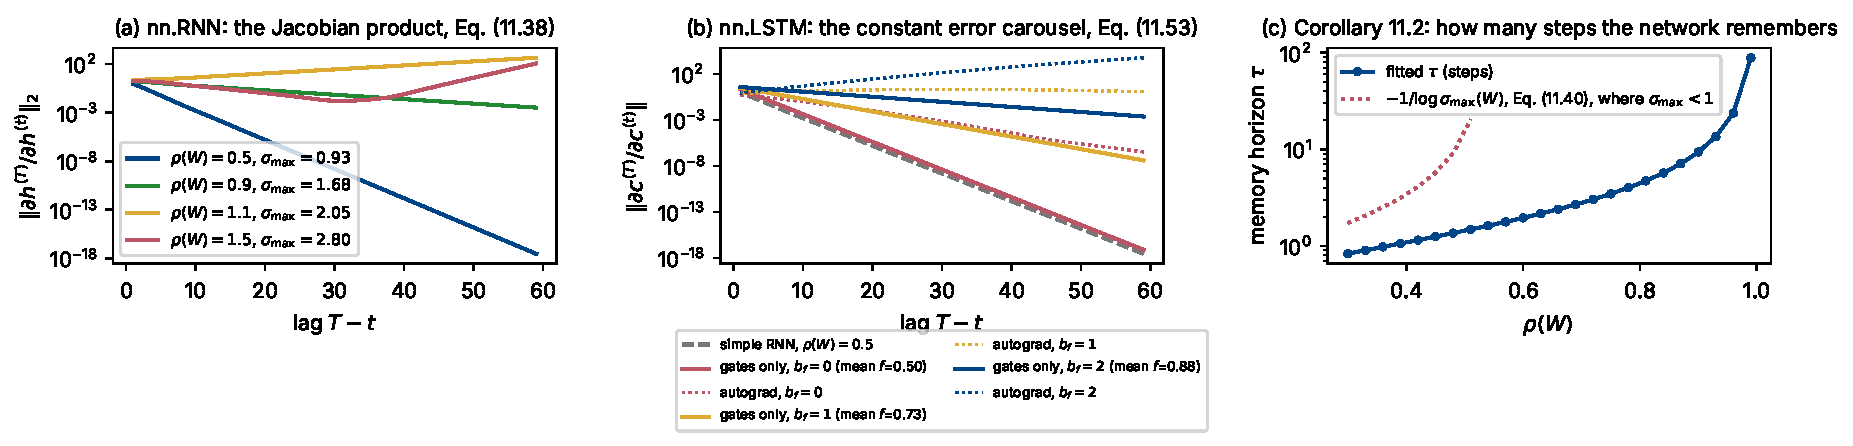
\includegraphics[width=\textwidth]{week45rnn_gradients}
\end{center}
\small
$n_h=20$, $T=60$, inputs small enough that $\tanh'\approx1$, $\bm{W}$ scaled
to a prescribed spectral radius; each curve is
\texttt{torch.autograd.functional.jacobian} of $\bm{h}^{(T)}$ with respect to
$\bm{h}^{(t)}$.  (a) At $\rho(\bm{W})=0.5$ the influence of the first step on
the last has fallen by \emph{eighteen orders of magnitude} over $59$ steps.
At $\rho=1.1$ it has grown to $450$.  (b) is for Part 6.  (c) The horizon
$\tau$ fitted to the slope of (a).
\end{frame}

\begin{frame}[fragile]{The numbers behind the figure}
\begin{lstlisting}
 rho(W)  sigma_max  mean max(tanh')   ||dh_T/dh_1||   bound sigma_max^59   fitted tau
  0.50     0.933        1.0000          2.878e-18        1.705e-02           1.44
  0.90     1.680        1.0000          3.313e-03        1.963e+13           9.38
  1.10     2.053        1.0000          4.547e+02        2.721e+18         -10.63
  1.50     2.800        0.9980          1.152e+02        2.410e+26         -20.40

 fitted memory horizon and the lag at which the influence has fallen by 1e-6:
   rho=0.50  tau=  1.44 steps   lag(1e-6)=  20
   rho=0.70  tau=  2.79         lag(1e-6)=  39
   rho=0.90  tau=  9.38         lag(1e-6)= 130
   rho=0.99  tau= 88.88         lag(1e-6)=1228
\end{lstlisting}
\small
The code that produced this is a dozen lines of the notebook: build the
layer, scale \texttt{weight\_hh\_l0}, run it, and ask autograd for the
Jacobian from each intermediate state to the last.
\end{frame}

\begin{frame}{Reading the table}
\begin{itemize}
  \item At $\rho(\bm{W})=0.5$ the memory horizon is \emph{one and a half
        steps}.  A network initialised this way has forgotten its input
        after two steps, and no amount of training on long sequences will
        change that until the weights themselves grow.
  \item The bound uses $\sigma_{\max}(\bm{W})$, not $\rho(\bm{W})$, and the
        two differ: $\rho=0.5$ has $\sigma_{\max}=0.93$, $\rho=0.9$ has
        $\sigma_{\max}=1.7$.  Between $\rho<1<\sigma_{\max}$ there is a
        regime of \emph{transient growth with asymptotic decay} -- the
        red curve of (a).  That is where carefully initialised recurrent
        networks actually operate.
  \item None of this depends on the library.  Autograd computes the product
        of Eq.~(11.38) exactly; the vanishing gradient is \emph{a property
        of the composition}, not of an implementation.
\end{itemize}
\end{frame}

\begin{insight}[two bits per step]
\question{(a) Show that the logistic function has $\max|\sigma'|=1/4$
and $\tanh$ has $\max|\tanh'|=1$.  (b) With $\tanh$, what is the horizon
$\tau$ of Eq.~(11.40) for $\sigma_{\max}(\bm{W})=0.9$, $0.99$ and $0.999$,
and how large must $\sigma_{\max}$ be for a horizon of $100$ steps?
(c) What does the theorem then say about the other side?}
\answer{(a) $\sigma'=\sigma(1-\sigma)$ is largest at $\sigma=1/2$, where it
is $1/4$; $\tanh'=1-\tanh^2$ is largest at $0$, where it is $1$.
(b) $\tau=-1/\log\sigma_{\max}$: $9.5$, $99.5$ and $999.5$ steps.  A
horizon of $100$ needs $\sigma_{\max}\ge e^{-1/100}\approx0.990$.
(c) The theorem's growth condition is $\mu\sigma_{\max}>1$, and $0.99$ sits
one per cent below it.  To remember a hundred steps the simple RNN must be
tuned to within a per cent of the exploding regime -- and training moves
$\bm{W}$.  That is the design problem the LSTM of Part 6 solves.}
\end{insight}

\begin{frame}{Gradient clipping, Eq.~(11.46)}
Vanishing and exploding gradients are not symmetric problems.  Explosion is
the easier of the two, because it is \emph{visible}: the gradient norm
spikes and the parameters jump.  The standard fix rescales any gradient
whose norm exceeds a threshold, keeping the direction:
\[
  \bm{g}\longleftarrow
  \begin{cases}
    \bm{g}, & \|\bm{g}\|\le\theta,\\[2pt]
    \dfrac{\theta}{\|\bm{g}\|}\,\bm{g}, & \|\bm{g}\|>\theta.
  \end{cases}
\]
\begin{block}{Proposition 11.3: clipping is a trust region}
(i) $\tilde{\bm{g}}=\lambda\bm{g}$ with $\lambda\in(0,1]$, so
$-\tilde{\bm{g}}$ is still a descent direction.  (ii) $\tilde{\bm{g}}$ is
the projection of $\bm{g}$ onto the ball of radius $\theta$, Eq.~(11.47),
so a step $\gamma\tilde{\bm{g}}$ never moves the parameters further than
$\gamma\theta$ -- the guarantee of a trust-region method, for free.
\end{block}
\end{frame}

\begin{frame}{Clipping: what it does not do, and where it lives}
\begin{block}{What it does not do}
Nothing whatever for \emph{vanishing} gradients: rescaling $10^{-18}$
upwards would amplify rounding noise, not signal.  Vanishing gradients need
a change of architecture (Part 6).
\end{block}
\begin{block}{In the libraries}
\texttt{Adam(lr, clipnorm=1.0)} in Keras;
\texttt{nn.utils.clip\_grad\_norm\_(model.parameters(), 1.0)} between
\texttt{backward()} and \texttt{step()} in PyTorch.  Both act on the
\emph{whole} gradient vector, all arrays jointly.
\end{block}
\begin{block}{Initialisation}
$\sigma_{\max}(\bm{W})\approx1$ puts the network at the edge between the
two regimes -- the best this architecture can do.  Orthogonal or identity
initialisations of $\bm{W}$ are attempts to sit exactly there.
\end{block}
\end{frame}

\begin{frame}{Clipping and initialization solve different problems}
\begin{columns}[T]
\begin{column}{0.49\textwidth}
\begin{block}{Clipping, Eq.~(11.46)}
Rescales the concatenated gradient to norm $\theta$ when it exceeds
$\theta$: the direction is preserved, a plain SGD step is bounded by
$\gamma\theta$, and a rare explosion cannot destroy the weights.  It does
\textbf{not} restore a contribution that has vanished: a factor $10^{-18}$
is still $10^{-18}$ after clipping.
\end{block}
\end{column}
\begin{column}{0.49\textwidth}
\begin{block}{Initialization}
An orthogonal $\bm{W}$ preserves norms in a \emph{linear} recurrence (all
singular values one).  With $\tanh$ the factors $\bm{D}^{(t)}$ still
contract, and unconstrained updates destroy the orthogonality within a few
steps.  It helps at the start; it is not a guarantee.  Check the input scale
and the saturation alongside $\bm{W}$ (previous frames).
\end{block}
\end{column}
\end{columns}
\begin{block}{The honest summary}
Clipping is for explosion.  For vanishing there is no fix inside the simple
RNN -- only the architectural change of the next part, or the attention
mechanism of Chapter 13.
\end{block}
\end{frame}


\begin{frame}{Four effective ways to train a recurrent network}
\begin{enumerate}
  \item \textbf{Long short-term memory.}  Make the RNN out of modules
        designed to remember values for a long time -- Part 6.
  \item \textbf{Hessian-free optimisation.}  An optimiser that can detect
        directions with a tiny gradient but an even smaller curvature
        (Newton's method of week 37 made affordable).
  \item \textbf{Echo-state networks.}  Initialise the recurrent
        connections very carefully, so that the hidden state is a reservoir
        of weakly coupled oscillators -- and learn only the read-out $\bm{V}$
        (linear regression, week 35!).
  \item \textbf{Good initialisation with momentum.}  Initialise as in an
        echo-state network, then learn everything, with momentum and
        clipping.
\end{enumerate}
\medskip
In practice: a gated cell, $\sigma_{\max}(\bm{W})\approx1$ at the start,
Adam, and clipping.  Before we gate anything, let us see what the plain
layer can do when the sequences are short enough.
\end{frame}

\begin{frame}[fragile]{The oscillator experiment, 1: the data and the Keras model (Section 11.6.1)}
\begin{lstlisting}
def make_windows(x, L=40, stride=5):           # x: one trajectory of 800 points
    idx = range(0, len(x) - L - 1, stride)
    X = np.stack([x[i:i + L] for i in idx])[..., None]        # (152, 40, 1): inputs x_i..x_{i+39}
    Y = np.stack([x[i + 1:i + L + 1] for i in idx])[..., None] # (152, 40, 1): targets, one step ahead
    return X, Y

model = keras.Sequential([keras.Input(shape=(None, 1)),
                          layers.SimpleRNN(24, return_sequences=True),
                          layers.Dense(1)])
model.compile(optimizer=keras.optimizers.Adam(5e-3, clipnorm=1.0), loss="mse")
model.fit(X_train, Y_train, epochs=300, batch_size=4, verbose=0)
\end{lstlisting}
\small
\begin{itemize}
  \item Data: the \emph{single} RK4 trajectory of panel (a), $\eta=0.2$,
        $(x_0,v_0)=(1,0)$, $800$ points -- the network sees only $x(t)$.
  \item Task: one-step-ahead forecasting at every step, along $152$
        overlapping windows of length $40$ (stride $5$).
  \item Network: $n_h=24$, $649$ parameters; Adam at $5\cdot10^{-3}$,
        clipping at $1$, $300$ epochs.
\end{itemize}
\end{frame}

\begin{frame}[fragile]{The oscillator experiment, 2: the same in PyTorch}
\begin{lstlisting}
model = Forecaster()                       # nn.RNN(1, 24) + nn.Linear(24, 1) from Part 3
opt, lossfn = torch.optim.Adam(model.parameters(), lr=5e-3), nn.MSELoss()
gnorms = []
for epoch in range(300):
    for idx in torch.randperm(len(X_train)).split(4):
        opt.zero_grad()
        loss = lossfn(model(X_train[idx]), Y_train[idx])
        loss.backward()
        gnorms.append(float(nn.utils.clip_grad_norm_(model.parameters(), 1.0)))
        opt.step()
\end{lstlisting}
\small
\begin{block}{The tests}
(b) the trajectory from $(0,1)$ -- a different solution of the same
equation, out of phase with everything the network saw; (c) an oscillator
driven by $F(t)=0.3\cos(0.7t)$ from $(0.5,-0.3)$, which the network never saw
in any form.  The split is by whole trajectories: every test trajectory has
a new initial condition.
\end{block}
\end{frame}

\begin{frame}{Two rules for sequential data}
\begin{block}{No shuffling across time}
Training and test \emph{windows} may be shuffled, the points inside a
window may not -- shuffling in time decorrelates the series and leaks the
future into the past.  \texttt{randperm(...).split(4)} and Keras's
\texttt{shuffle=True} shuffle windows, never steps.
\end{block}
\begin{block}{The cost}
Mean squared error of predicted against actual trajectory, Eq.~(11.5): a
forecasting problem is a regression problem, and we are free to choose
among the regression losses of week 35.
\end{block}
\end{frame}

\begin{frame}[fragile]{The result (\texttt{week45rnn\_oscillator.pdf})}
\begin{center}
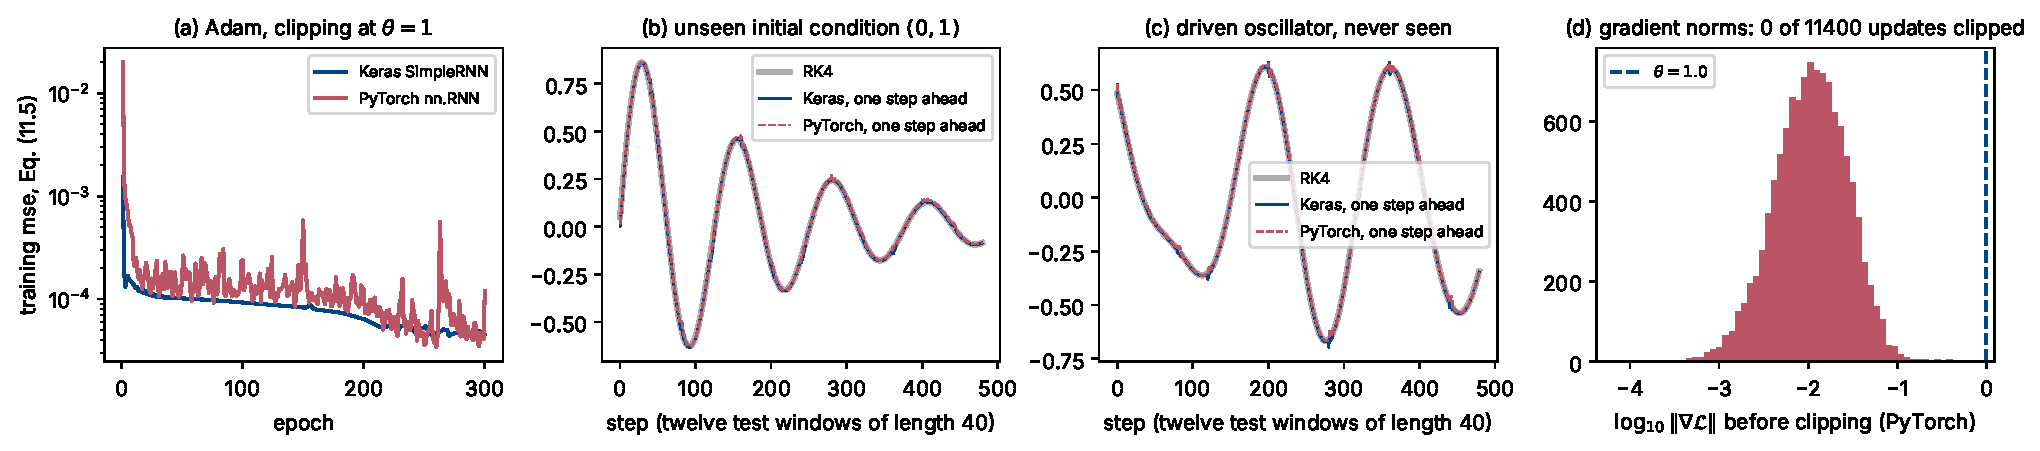
\includegraphics[width=0.95\textwidth]{week45rnn_oscillator}
\end{center}
\begin{lstlisting}
 set          Keras mse   PyTorch mse   Var(x)   relative (Keras / PyTorch)
 train       3.692e-05    1.056e-04   0.0655   0.056% / 0.161%
 unseen IC   3.811e-05    1.023e-04   0.0618   0.062% / 0.166%
 driven      4.970e-05    1.269e-04   0.1488   0.033% / 0.085%
 PyTorch gradient norms before clipping: median 0.011, max 0.77, 0 of 11400 updates clipped
\end{lstlisting}
\end{frame}

\begin{frame}{What the result says}
\begin{itemize}
  \item The second row is the interesting one: trained on a trajectory
        starting from rest at unit displacement, tested on one starting from
        the origin at unit velocity, the error is \emph{the same as the
        training error} -- six parts in ten thousand of the variance in
        Keras, sixteen in PyTorch.
  \item The driven oscillator, never seen, is predicted just as well.
  \item The network has not memorised a trajectory; it has learned a
        \emph{one-step update rule}, as Eq.~(11.12) said it would -- the same
        payoff parameter sharing gave in week 44.  Whether that rule is the
        oscillator's, or merely ``next value $\approx$ this value'', the
        one-step test cannot say: the free rollout three frames on can.
  \item The two libraries differ by a factor of three in the final error:
        different random initialisations and different batch orderings.
        Both are far below anything that matters.
  \item (d): with $\sigma_{\max}(\bm{W})\approx1$ at the start and sequences
        of $40$ steps, clipping never fired in $11\,400$ updates.  It is
        insurance.
\end{itemize}
\end{frame}

\begin{frame}{Why a good one-step fit can fail in a rollout (Section 11.6.2, Eq.~(11.48))}
At training time the network receives \emph{measured} states; in a
\emph{free rollout} it feeds back its own predictions.  With
$\bm{e}_t=\hat{\bm{s}}_t-\bm{s}_t$ and the local model discrepancy
$\bm{r}_t=\hat f(\bm{s}_t,F_t)-f(\bm{s}_t,F_t)$, to first order
\[
  \bm{e}_{t+1}\simeq\bm{J}_{\hat f}(\bm{s}_t,F_t)\,\bm{e}_t+\bm{r}_t .
\]
\begin{block}{Two sources, one curve}
The rollout \emph{injects} new error ($\bm{r}_t$) at every step and
\emph{transports} the old one ($\bm{J}_{\hat f}\bm{e}_t$) -- the same
Jacobian that governed the gradients now governs the forecast.  A small
one-step test loss says nothing about phase, amplitude or timing after many
periods.
\end{block}
\begin{block}{What to do}
Validate on held-out trajectories; plot the error \emph{against the forecast
horizon}; compare one-step evaluation with a free rollout under the same
forcing; and compare with a trusted reference (RK4), not with the Euler data
of a different integrator.  The next frame does this for the oscillator
network we just trained.
\end{block}
\end{frame}

\begin{frame}[fragile]{Measured: closing the loop (\texttt{week45rnn\_rollout.pdf})}
\begin{center}
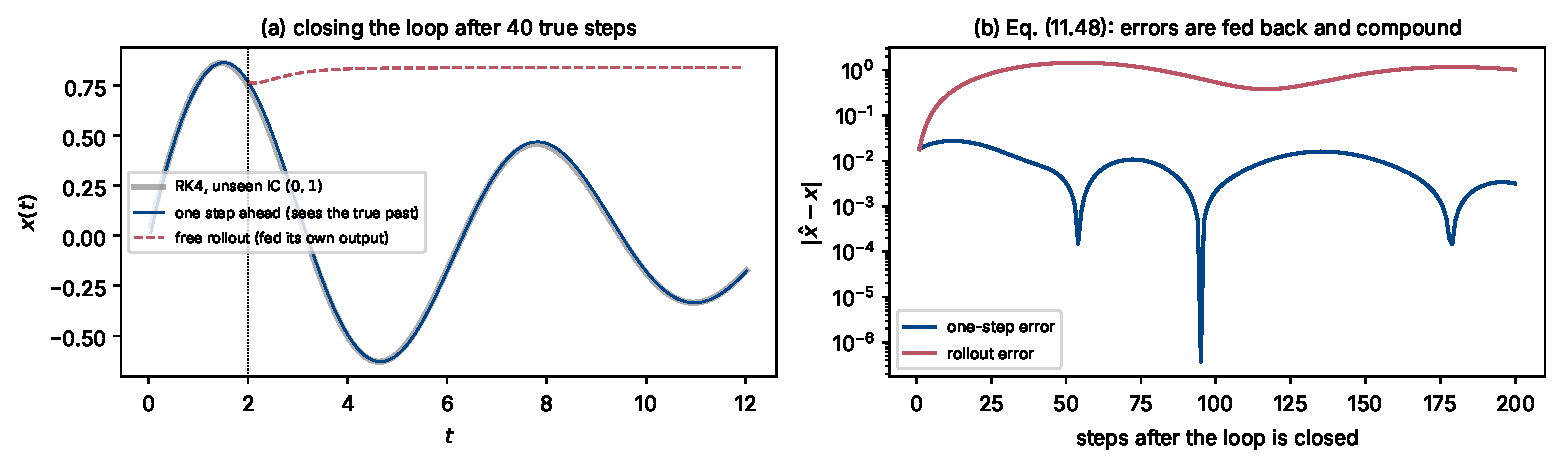
\includegraphics[width=0.86\textwidth]{week45rnn_rollout.pdf}
\end{center}
\vspace{-4pt}
\begin{columns}[T]
\begin{column}{0.42\textwidth}
\begin{lstlisting}
_, h = model(x_true[:40])   # warm-up on truth
x = x_true[39]
for _ in range(200):        # close the loop
    x, h = model(x, h)      # own output fed back
\end{lstlisting}
\end{column}
\begin{column}{0.56\textwidth}
\scriptsize
The same \texttt{nn.RNN} forecaster, on the unseen initial condition.  Fed
the true past it tracks RK4 to $10^{-2}$ (median one-step error
$8\times10^{-3}$).  Fed its own output it \textbf{freezes at a constant
within twenty steps}: at $\Delta t=0.05$ a map close to the identity already
has a tiny one-step loss, and nothing in the training ever checked whether
the network carried the \emph{velocity} in $\bm{h}$.  The ``learned rule''
of the previous frames is a one-step rule; the free rollout is the test it
had not been given.  The remedies are in the training, not in the cell:
predict increments, train on multi-step rollouts (truncated BPTT through
the network's own outputs), or give the network the state it is missing.
\end{column}
\end{columns}
\end{frame}

\begin{frame}{A diagnostic for each failure mode}
\small
\begin{center}
\begin{tabular}{p{4.4cm}p{8.4cm}}\toprule
observation & measurement or controlled comparison\\\midrule
only short-delay cases work & vary the delay on the copy task; track the gradient of the final loss at each earlier state (\texttt{torch.autograd}, as in \texttt{week45rnn\_gradients.pdf})\\[3pt]
loss spikes intermittently & log the global gradient norm \emph{before} clipping, the clipping fraction and the update norms (panel (d) of \texttt{week45rnn\_oscillator.pdf})\\[3pt]
many hidden units near $\pm1$ & inspect the distribution of $1-h^{(t)2}_i$; rescale the inputs\\[3pt]
results depend on chunk boundaries & vary the chunk length with the task and the loss normalization fixed\\[3pt]
one-step errors small but rollouts drift & compare phase and amplitude over increasing horizons on held-out trajectories, against a trusted integrator\\\bottomrule
\end{tabular}
\end{center}
Every row is a measurement, not a guess: this is how to debug a recurrent
network in a project.
\end{frame}


%% =====================================================================
\section{Long short-term memory}
\begin{frame}{The idea: a memory cell with gates (Section 11.7)}
\begin{columns}[T]
\begin{column}{0.5\textwidth}
Theorem 11.1 says the trouble is a product of Jacobians, each carrying a
factor $\bm{W}$ and a factor $\sigma_h'$.  Any architecture that keeps the
gradient alive over long lags must \emph{break that product}.

\medskip
Hochreiter and Schmidhuber (1997) did so with a second state variable whose
update is \emph{additive} -- a memory cell:
\begin{itemize}
  \item a linear unit with a self-connection of weight $1$ maintains its
        value indefinitely;
  \item information is written when a \emph{write} gate opens, kept while a
        \emph{keep} gate is open, read when a \emph{read} gate opens.
\end{itemize}
The gates are logistic functions, hence differentiable, so the whole
circuit trains by backpropagation.
\end{column}
\begin{column}{0.48\textwidth}
\begin{center}
\includegraphics[width=0.9\textwidth]{LSTM2}\\
\scriptsize The LSTM cell of Raschka et al.: the horizontal line at the top
carries $\bm{c}^{(t-1)}$ to $\bm{c}^{(t)}$; the four yellow boxes are the
gates.
\end{center}
\end{column}
\end{columns}
\end{frame}

\begin{frame}{The forget gate, Eq.~(11.49)}
\begin{columns}[T]
\begin{column}{0.5\textwidth}
\[
  \bm{f}^{(t)}=\sigma\!\left(\bm{W}_{fx}\bm{x}^{(t)}+\bm{W}_{fh}\bm{h}^{(t-1)}+\bm{b}_f\right).
\]
The logistic $\sigma$ is near $0$ for very negative arguments and near $1$
for very positive ones: $\bm{f}^{(t)}$ is a soft, learned, per-component
switch on the long-term memory.

\medskip
The name is slightly off -- $f=1$ means \emph{keep}.
\end{column}
\begin{column}{0.48\textwidth}
\begin{center}
\includegraphics[width=0.95\textwidth]{LSTM6}
\end{center}
\end{column}
\end{columns}
\end{frame}

\begin{frame}{The input gate, Eq.~(11.50)}
Two functions rather than one -- a logistic deciding \emph{how much} and a
$\tanh$ deciding \emph{what}:
\[
\begin{aligned}
  \bm{i}^{(t)}&=\sigma\!\left(\bm{W}_{ix}\bm{x}^{(t)}+\bm{W}_{ih}\bm{h}^{(t-1)}+\bm{b}_i\right),\\
  \bm{g}^{(t)}&=\tanh\!\left(\bm{W}_{gx}\bm{x}^{(t)}+\bm{W}_{gh}\bm{h}^{(t-1)}+\bm{b}_g\right).
\end{aligned}
\]
$\bm{g}^{(t)}$ is a candidate value in $(-1,1)$ -- exactly the simple RNN
update -- and $\bm{i}^{(t)}$ decides how much of it is written.
\end{frame}

\begin{frame}{The cell update, Eq.~(11.51): the whole idea in one line}
With $\odot$ the elementwise product,
\[
  \boxed{\;\bm{c}^{(t)}=\bm{f}^{(t)}\odot\bm{c}^{(t-1)}+\bm{i}^{(t)}\odot\bm{g}^{(t)}.\;}
\]
\begin{block}{Read it slowly}
Multiplied once (by the forget gate), added to once (by the input gate).
No weight matrix, no squashing function on the path from $\bm{c}^{(t-1)}$ to
$\bm{c}^{(t)}$.
\end{block}
\end{frame}

\begin{frame}{The output gate, Eq.~(11.52), and the cost of all this}
\begin{columns}[T]
\begin{column}{0.5\textwidth}
\[
\begin{aligned}
  \bm{o}^{(t)}&=\sigma\!\left(\bm{W}_{ox}\bm{x}^{(t)}+\bm{W}_{oh}\bm{h}^{(t-1)}+\bm{b}_o\right),\\
  \bm{h}^{(t)}&=\bm{o}^{(t)}\odot\tanh\!\left(\bm{c}^{(t)}\right).
\end{aligned}
\]
$\bm{h}^{(t)}$ is both the output of the cell (what the read-out sees) and
the input to the next time step.

\medskip
Four gates, each with its own $\bm{W}_{\cdot x}$, $\bm{W}_{\cdot h}$ and
bias: \textbf{four times the parameters} of a simple RNN with the same
$n_h$, $4n_h(n_x+n_h+1)$ -- the $2496$ against $624$ of Part 3.
\end{column}
\begin{column}{0.48\textwidth}
\begin{center}
\includegraphics[width=0.95\textwidth]{LSTM9}
\end{center}
\end{column}
\end{columns}
\end{frame}

\begin{frame}{The circuit, and the constant error carousel (Figure 11.5)}
\begin{center}
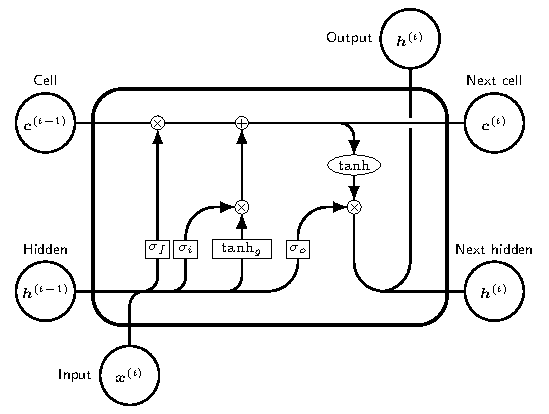
\includegraphics[width=0.5\textwidth]{lstmcell}
\end{center}
Follow the horizontal line entering as $\bm{c}^{(t-1)}$ and leaving as
$\bm{c}^{(t)}$: it meets one multiplication and one addition and nothing
else.  Every other path hangs \emph{off} that line.  The simple RNN would
have the state line running through a matrix multiplication and a $\tanh$
at every step.  The LSTM did not remove those operations; it \emph{moved
them off the memory path}.
\end{frame}

\begin{frame}{Why it works, Eq.~(11.53)}
Differentiate the cell update with respect to the previous cell state,
treating the gates as slowly varying:
\[
  \frac{\partial\bm{c}^{(t)}}{\partial\bm{c}^{(t-1)}}\approx\operatorname{diag}\!\left(\bm{f}^{(t)}\right),
  \qquad
  \frac{\partial\bm{c}^{(T)}}{\partial\bm{c}^{(t)}}\approx\prod_{k=t+1}^{T}\operatorname{diag}\!\left(\bm{f}^{(k)}\right).
\]
Compare Eq.~(11.38): no $\bm{W}$, no $\sigma_h'$ -- the product is over the
forget gates alone.  If the network learns to hold $f\approx1$ on some
component, the gradient along it travels essentially undamped for as long
as the gate stays open.  That is the \emph{constant error carousel}.

\medskip
It is worth checking, because the argument is often stated as though the
LSTM simply solves the problem -- and it does not.
\end{frame}

\begin{frame}[fragile]{Measured on an untrained \texttt{nn.LSTM} (panel (b) of \texttt{week45rnn\_gradients.pdf})}
$n_h=20$, $T=60$; the forget-gate bias set through
\texttt{lstm.bias\_ih\_l0[n\_h:2n\_h] = b\_f}.  Two numbers per bias: the
product of forget gates read from the layer, Eq.~(11.53), and the exact
Jacobian $\partial\bm{c}^{(T)}/\partial\bm{c}^{(1)}$ from autograd
(Proposition 11.4):
\begin{lstlisting}
 forget bias   mean f   gate product (11.53)   exact autograd (Prop. 11.4)
        0.0    0.5000       7.759e-18               3.493e-07       (simple RNN, rho=0.5: 2.9e-18)
        1.0    0.7311       4.202e-08               1.269e+00
        2.0    0.8803       2.435e-03               6.026e+03
\end{lstlisting}
\small
\begin{itemize}
  \item With $\bm{b}_f=0$ the gates sit at $\sigma(0)=1/2$, the product is
        $2^{-59}\approx10^{-18}$: along the cell path alone the LSTM is
        \emph{no better than the simple RNN it was invented to replace}.
  \item Biasing the gates open buys ten orders of magnitude at $b_f=1$ and
        fifteen at $b_f=2$.
  \item The exact Jacobian is larger still: the gates conduct too.  At
        $b_f=1$ it is of order \emph{one} -- a gradient that survives sixty
        steps intact -- and at $b_f=2$ it is $6000$: nothing here prevents
        explosion, so clipping stays.
\end{itemize}
\end{frame}

\begin{insight}[the forget-gate bias]
\question{PyTorch's \texttt{nn.LSTM} draws all biases uniformly from
$(-1/\sqrt{n_h},1/\sqrt{n_h})$; Keras's \texttt{LSTM} has
\texttt{unit\_forget\_bias=True} by default.  Where does the mean forget
gate start in each, what does the table predict, and what would you do
about it in PyTorch?}
\answer{PyTorch: the bias is essentially zero, so $f\approx\sigma(0)=1/2$
and the cell path transmits $2^{-59}\approx10^{-18}$ -- the first line of
the table.  Keras: $b_f=1$, $f\approx0.73$ -- the second line, ten orders of
magnitude better along the cell path and a Jacobian of order one in full.
In PyTorch, one line after constructing the layer:
\texttt{with torch.no\_grad(): lstm.bias\_ih\_l0[n\_h:2*n\_h] = 1.0}
(gate order $\bm{i},\bm{f},\bm{g},\bm{o}$).  Jozefowicz et al.\ (2015) found
this among the most reliable single adjustments -- and on the spoken digits
it will buy almost two percentage points.  The architecture
supplies a \emph{path}; the initialisation decides whether training starts
anywhere near it.}
\end{insight}

\begin{frame}[fragile]{LSTM and GRU in the two libraries}
\begin{lstlisting}
# Keras: one word changes
model = keras.Sequential([keras.Input(shape=(T, n_x)), layers.LSTM(64), layers.Dense(10)])
#        ...                                            layers.GRU(64)   ...
# PyTorch: same calls, one more output
lstm = nn.LSTM(n_x, 64, batch_first=True)
H, (h_T, c_T) = lstm(x)             # H: (N, T, 64) = every h_t;  h_T, c_T: (1, N, 64)
with torch.no_grad():
    lstm.bias_ih_l0[64:128] = 1.0   # forget gate open at the start, as Keras does
gru = nn.GRU(n_x, 64, batch_first=True)
H, h_T = gru(x)                     # no cell state
\end{lstlisting}
\small
\begin{itemize}
  \item Inside, both libraries compute the four gates with \emph{one}
        matrix multiplication on $(\bm{x}^{(t)},\bm{h}^{(t-1)})$ and split the
        result: \texttt{weight\_ih\_l0} has shape $(4n_h,n_x)$, in the order
        $(\bm{i},\bm{f},\bm{g},\bm{o})$.
  \item \texttt{return\_state=True} in Keras gives $(\bm{h}^{(T)},\bm{c}^{(T)})$
        too; pass them as \texttt{initial\_state} to continue a sequence.
  \item Everything else -- the read-out, the loss, clipping, the training
        loop -- is unchanged from the simple RNN.
\end{itemize}
\end{frame}

\begin{frame}{The gated recurrent unit, Eq.~(11.56)}
Cho et al.\ (2014) apply the same idea with fewer parts: no separate cell
state, two gates instead of three,
\[
\begin{aligned}
  \bm{z}^{(t)}&=\sigma\!\left(\bm{W}_{zx}\bm{x}^{(t)}+\bm{W}_{zh}\bm{h}^{(t-1)}+\bm{b}_z\right),\\
  \bm{r}^{(t)}&=\sigma\!\left(\bm{W}_{rx}\bm{x}^{(t)}+\bm{W}_{rh}\bm{h}^{(t-1)}+\bm{b}_r\right),\\
  \tilde{\bm{h}}^{(t)}&=\tanh\!\left(\bm{W}_{hx}\bm{x}^{(t)}+\bm{W}_{hh}\left(\bm{r}^{(t)}\odot\bm{h}^{(t-1)}\right)+\bm{b}_h\right),\\
  \bm{h}^{(t)}&=\left(1-\bm{z}^{(t)}\right)\odot\bm{h}^{(t-1)}+\bm{z}^{(t)}\odot\tilde{\bm{h}}^{(t)}.
\end{aligned}
\]
The \emph{update} gate $\bm{z}$ is forget and input gate at once -- what is
not written is retained, by construction; the \emph{reset} gate $\bm{r}$
controls how much of the past enters the candidate.  The last line has the
additive form of Eq.~(11.51), so the carousel argument applies with
$1-\bm{z}$ in place of $\bm{f}$.
\end{frame}

\begin{frame}{LSTM or GRU, and what came after}
\begin{block}{Cost and performance}
Three sets of matrices against the LSTM's four: three quarters of the
parameters and the computation ($1944$ against $2496$ in Part 3).  Which is
better is task-dependent and not settled; the two are usually close (Chung
et al.\ 2014, Jozefowicz et al.\ 2015).
\end{block}
\begin{block}{Still moving}
Beck et al.\ (2024, xLSTM): exponential gating and modified memory
structures make an extended LSTM competitive with transformers and
state-space models.  The transformer itself, which replaces recurrence by
attention, is Chapter 13.
\end{block}
\end{frame}

%% =====================================================================
\section{Four applications}
\begin{frame}[fragile]{Forecasting a sine wave, 1: Keras (Section 11.8.1)}
\begin{lstlisting}
time_steps = np.linspace(0, 100, 500); data = np.sin(time_steps); seq_length = 20
X = np.array([data[i:i+seq_length] for i in range(len(data)-seq_length)]).reshape(-1, seq_length, 1)
y = data[seq_length:].reshape(-1, 1)                       # the next value after each window
split = int(0.8 * len(X))                                  # split in TIME, not at random

model = keras.Sequential([keras.Input(shape=(seq_length, 1)),
                          layers.SimpleRNN(16),            # last state only: (N, 16)
                          layers.Dense(1)])
model.compile(optimizer=keras.optimizers.Adam(1e-2, clipnorm=1.0), loss="mse")
model.fit(X[:split], y[:split], epochs=200, batch_size=32, verbose=0,
          validation_data=(X[split:], y[split:]))
\end{lstlisting}
\small
Sequence-to-label: $20$ values in, \emph{one} value out, so
\texttt{return\_sequences} stays at its default \texttt{False} and
\texttt{Dense(1)} acts on the last state.  The last $20\%$ of the wave is
the test set.
\end{frame}

\begin{frame}[fragile]{Forecasting a sine wave, 2: PyTorch}
\begin{lstlisting}
class SineRNN(nn.Module):
    def __init__(self, hidden=16):
        super().__init__()
        self.rnn = nn.RNN(input_size=1, hidden_size=hidden, batch_first=True)
        self.fc = nn.Linear(hidden, 1)
    def forward(self, x):
        out, h_T = self.rnn(x)                 # out: (N, 20, 16), every h_t
        return self.fc(out[:, -1, :])          # read out the last state only

model = SineRNN(); opt = torch.optim.Adam(model.parameters(), lr=1e-2); lossfn = nn.MSELoss()
for epoch in range(200):
    for idx in torch.randperm(split).split(32):
        opt.zero_grad()
        loss = lossfn(model(X[idx]), y[idx])
        loss.backward()
        nn.utils.clip_grad_norm_(model.parameters(), 1.0)
        opt.step()
\end{lstlisting}
\small
\texttt{out[:, -1, :]} is Keras's \texttt{return\_sequences=False}.  The
loop is the one of Part 3, unchanged.
\end{frame}

\begin{frame}[fragile]{Both reach the same place (\texttt{week45rnn\_sine.pdf})}
\begin{center}
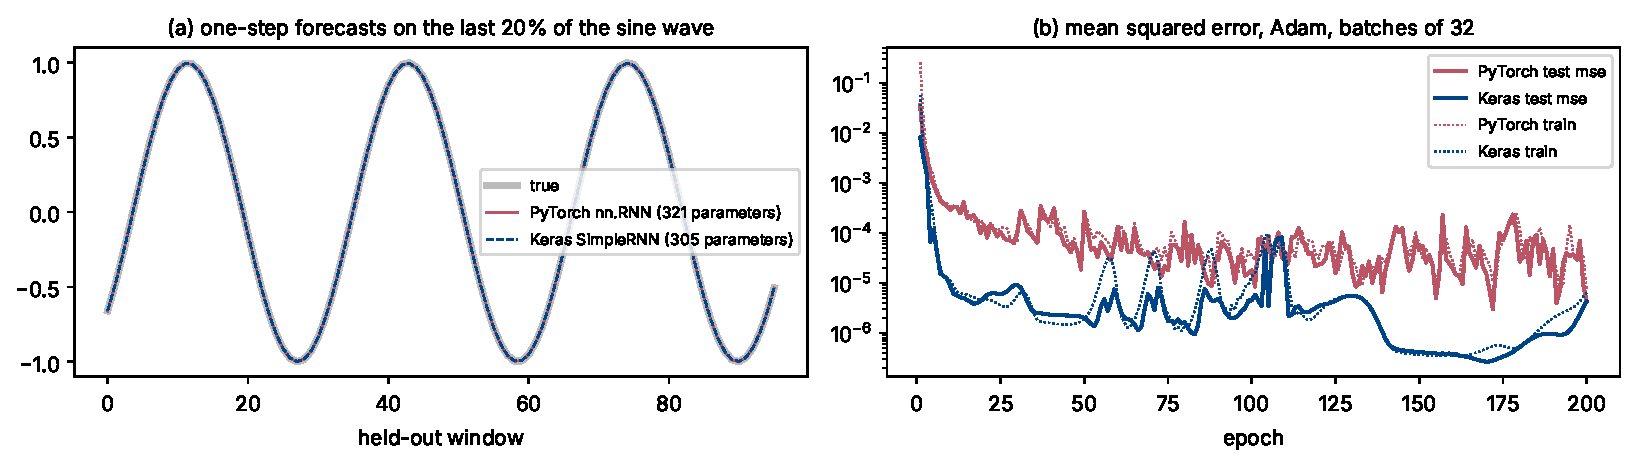
\includegraphics[width=0.9\textwidth]{week45rnn_sine}
\end{center}
\begin{lstlisting}
PyTorch    epoch 200: train mse 0.000008   test mse 0.000004   (321 parameters)
Keras      epoch 200: train mse 0.000006   test mse 0.000004   (305 parameters)
rms error on the held-out windows: 0.0021 (both), amplitude 1
\end{lstlisting}
\small
A test mean squared error of a few $10^{-6}$ is a root-mean-square error of
a few $10^{-3}$ on a signal of unit amplitude: both predictions lie on the
true curve.  The parameter counts differ by sixteen: the second bias vector.
\end{frame}

\begin{frame}[fragile]{MNIST read row by row (Section 11.8.2)}
Treat each $28\times28$ image as a sequence of $28$ rows, each of $28$
features, and classify it from the last state -- a sequence-to-label task.
Not what one does in practice (week 44 explains why a CNN is the right
tool), but a clean demonstration.
\begin{lstlisting}
# Keras
m = keras.Sequential([keras.Input(shape=(28, 28)), layers.LSTM(128), layers.Dense(10)])
m.compile(optimizer=keras.optimizers.Adam(1e-3, clipnorm=1.0),
          loss=keras.losses.SparseCategoricalCrossentropy(from_logits=True), metrics=["accuracy"])
m.fit(x_train, y_train, epochs=3, batch_size=64)        # x_train: (60000, 28, 28) in [0, 1]

# PyTorch
class RowNet(nn.Module):
    def __init__(self):
        super().__init__()
        self.rnn = nn.LSTM(28, 128, batch_first=True)    # 28 steps of 28 features
        self.fc = nn.Linear(128, 10)
    def forward(self, x):
        return self.fc(self.rnn(x)[0][:, -1, :])         # last state -> class scores
criterion = nn.CrossEntropyLoss()                        # softmax + cross entropy, week 41
\end{lstlisting}
\small The parameter count $4n_h(n_x+n_h+1)=80\,384$ printed by
\texttt{model.summary()} is the four-gates check of Part 3.
\end{frame}

\begin{frame}[fragile]{Row by row: the two libraries, two cells (\texttt{week45rnn\_mnist\_rows.pdf})}
\begin{columns}[T]
\begin{column}{0.5\textwidth}
\begin{center}
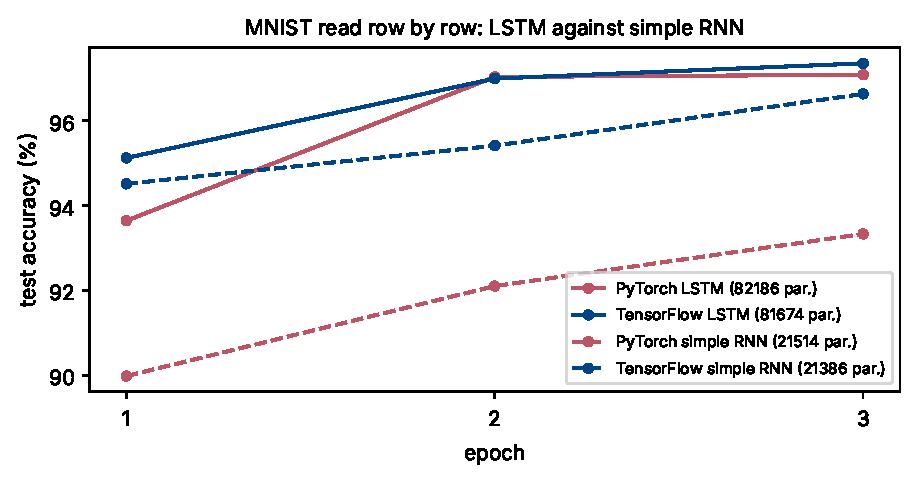
\includegraphics[width=\textwidth]{week45rnn_mnist_rows}
\end{center}
\end{column}
\begin{column}{0.5\textwidth}
\begin{lstlisting}
cell        framework   parameters  test acc.
LSTM        PyTorch          82186     0.9708
LSTM        Keras            81674     0.9735
simple RNN  PyTorch          21514     0.9333
simple RNN  Keras            21386     0.9663
\end{lstlisting}
\small Three epochs, Adam $10^{-3}$, batches of $64$, $n_h=128$, the full
$60\,000$ images; accuracy on the $10\,000$ test images.
\end{column}
\end{columns}
\begin{itemize}
  \item The LSTM beats the simple RNN on a task with only $28$ time steps --
        short enough that the simple RNN works, just less well.
  \item The whole exercise reaches about $0.97$, where the convolutional
        network of week 44 reached $0.99$: reading an image as a sequence
        throws away the vertical structure that a CNN was built to exploit.
\end{itemize}
\end{frame}

\begin{frame}{Sound: spoken digits (\texttt{week45rnn\_digits.pdf}, panels (a) and (b))}
\begin{center}
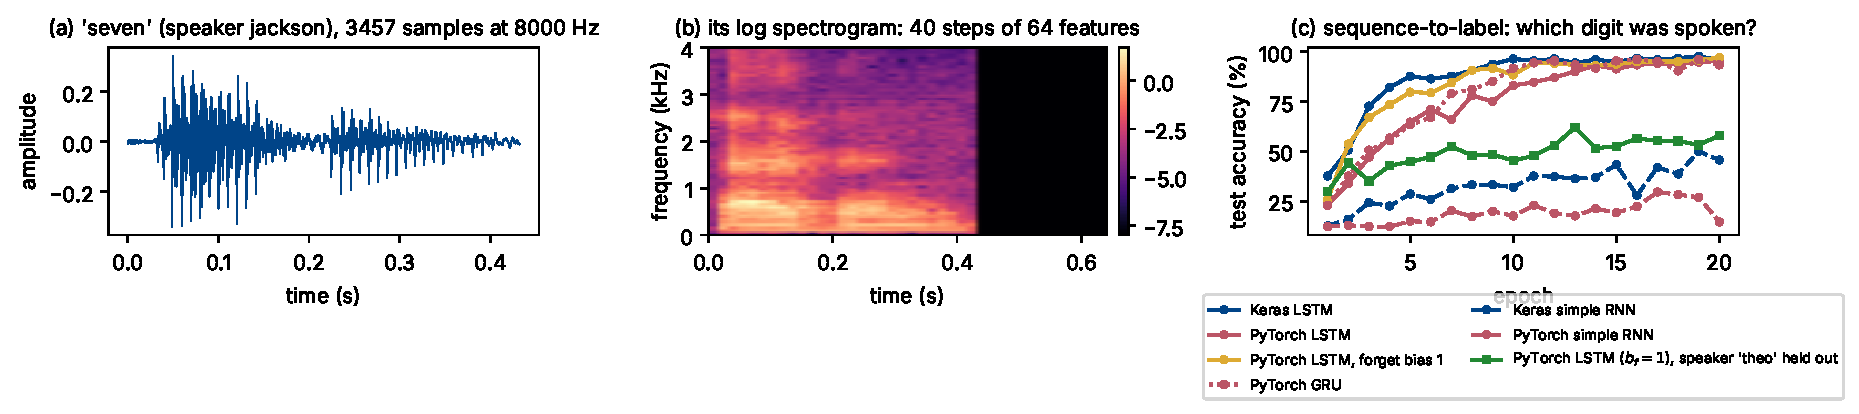
\includegraphics[width=\textwidth]{week45rnn_digits}
\end{center}
\small
The Free Spoken Digit Dataset: $3000$ recordings of the digits $0$--$9$ by
six speakers, $8$ kHz, $0.15$--$2$ s each (median $0.42$ s).  A real
sequence-to-label problem with sequences of different lengths, and the data
are \emph{sound}: the notebook plays them.
\end{frame}

\begin{frame}[fragile]{Sound: from a waveform to a sequence of feature vectors}
A waveform of $3457$ samples is too long a sequence for a simple recurrent
layer (Corollary 11.2), and the information in speech sits in how the
\emph{spectrum} changes with time.  So we do what every speech system does:
\begin{lstlisting}
def log_spectrogram(x, n_fft=256, hop=128, n_frames=40, n_bins=64):
    x = np.pad(x, (0, max(0, n_fft + hop*(n_frames-1) - len(x))))[:n_fft + hop*(n_frames-1)]
    frames = np.stack([x[i*hop:i*hop + n_fft] for i in range(n_frames)])   # 32 ms every 16 ms
    spec = np.abs(np.fft.rfft(frames * np.hanning(n_fft), axis=1)) ** 2    # (40, 129) power
    spec = spec[:, :2*n_bins].reshape(n_frames, n_bins, 2).mean(axis=2)    # (40, 64) bands
    return np.log10(spec + 1e-8).astype("float32")
\end{lstlisting}
\small
\begin{itemize}
  \item Frames of $32$ ms every $16$ ms, a Hann window, the power spectrum
        (Chapter 10, week 44: the Fourier transform of a windowed signal).
  \item $129$ frequency bins averaged in pairs to $64$ bands; logarithm
        because loudness is logarithmic; padded with silence or cut to $40$
        frames ($0.66$ s).
  \item The result is a 3-tensor $(3000,40,64)$: \emph{the data layout of
        Part 3}, $T=40$ steps of $n_x=64$ features -- panel (b).
\end{itemize}
\end{frame}

\begin{frame}[fragile]{Sound: the models, in both libraries}
\begin{lstlisting}
# Keras: 40 steps of 64 features in, 10 class scores out
m = keras.Sequential([keras.Input(shape=(40, 64)), layers.LSTM(64), layers.Dense(10)])
m.compile(optimizer=keras.optimizers.Adam(1e-3, clipnorm=1.0),
          loss=keras.losses.SparseCategoricalCrossentropy(from_logits=True), metrics=["accuracy"])
m.fit(X_train, y_train, epochs=20, batch_size=32, validation_data=(X_test, y_test))

# PyTorch
core, head = nn.LSTM(64, 64, batch_first=True), nn.Linear(64, 10)
with torch.no_grad():
    core.bias_ih_l0[64:128] = 1.0                        # the forget-gate bias of Pause 6
for epoch in range(20):
    for idx in torch.randperm(len(X_train)).split(32):
        opt.zero_grad()
        loss = nn.CrossEntropyLoss()(head(core(X_train[idx])[0][:, -1, :]), y_train[idx])
        loss.backward(); nn.utils.clip_grad_norm_(params, 1.0); opt.step()
\end{lstlisting}
\small
The dataset's standard split: recordings $0$--$4$ of each digit and speaker
are the test set ($300$), the rest train ($2700$).  One global
standardisation of the features.  Everything else is the MNIST code with
$28\to40$ steps and $28\to64$ features.
\end{frame}

\begin{frame}[fragile]{Sound: the results (panel (c))}
\begin{lstlisting}
 cell             framework   parameters   test accuracy   split
 LSTM             Keras           33674          0.9567   standard
 LSTM             PyTorch         33930          0.9533   standard
 LSTM, b_f = 1    PyTorch         33930          0.9700   standard
 GRU              PyTorch         25610          0.9333   standard
 simple RNN       Keras            8906          0.4567   standard
 simple RNN       PyTorch          8970          0.1467   standard
 LSTM, b_f = 1    PyTorch         33930          0.5800   speaker 'theo' held out
\end{lstlisting}
\small Adam $10^{-3}$, batches of $32$, $n_h=64$, $20$ epochs; $10$ classes,
so chance is $0.10$.
\end{frame}

\begin{frame}{Sound: reading the results}
\begin{itemize}
  \item A gated cell classifies a spoken digit from its spectrogram with
        $95$--$97\%$ accuracy after twenty epochs and half a minute of
        training.  The GRU is close behind with three quarters of the
        parameters.
  \item The simple RNN \emph{fails}: $15\%$ in PyTorch, $46\%$ in Keras,
        against a chance level of $10\%$.  Forty steps is beyond its memory
        horizon at initialisation, and the label depends on the whole
        utterance.  This is Corollary 11.2 on real data.
  \item The two libraries' LSTMs agree to within half a point; setting the
        forget-gate bias to one in PyTorch adds almost two points on top.
        Pause 6 made a prediction; this is the measurement.  (The Keras
        numbers move by a point or so between runs -- TensorFlow's threading
        is not seeded; the PyTorch numbers are reproducible.)
  \item Hold out one of the six \emph{speakers} instead of random
        recordings and the accuracy falls to $58\%$.  The standard split
        tests whether the network recognises digits \emph{from these
        speakers}; the speaker split tests whether it recognises digits.
\end{itemize}
\end{frame}

\begin{insight}[the held-out speaker]
\question{Why does accuracy fall from $97\%$ to $58\%$ when one speaker is
held out, and what does that say about the standard split?  Which of the
course's tools would you use to decide which number to report?}
\answer{In the standard split every test recording comes from a speaker
whose other $495$ recordings are in the training set: the network can use
the speaker's pitch, accent and tempo as features, and it does.  Held-out
recordings are therefore \emph{not independent} of the training data in
the sense that matters for generalisation to a new speaker -- the
i.i.d.\ assumption of the first frame, violated at the level of the split
rather than of the samples.  The honest estimate for a system meant to
work on new voices is the speaker split; with six speakers that is
\emph{leave-one-speaker-out cross-validation} (week 36), six folds, and
the number to report is the mean and its spread.  More speakers, data
augmentation (pitch and tempo shifts) and a bidirectional layer are the
usual ways to raise it.}
\end{insight}

\begin{frame}{The experiment the theory demands: the adding problem (Section 11.8.5)}
We have seen that the LSTM keeps a larger Jacobian, and classifies better
over $28$ and $40$ steps.  Neither is the claim the architecture was
invented to support: that gating lets a network learn dependencies a simple
recurrence \emph{cannot}.  Testing that needs a task where nothing but
long-range memory is measured.
\begin{block}{The adding problem}
Each sequence has two channels: the first carries values drawn uniformly
from $[0,1]$, the second is zero except for exactly two markers, one in
each half.  The target is half the sum of the two marked values.
\end{block}
Nothing can be inferred from local statistics -- the values are i.i.d.\ --
so a model must hold one number from the first half until the second marker
arrives, while ignoring everything in between.  Predicting the mean gives
a mean squared error of about $0.043$; that is the number to beat.
\end{frame}

\begin{frame}[fragile]{The adding problem: setup}
\begin{lstlisting}
for T in (10, 30, 60, 120):
    for Cell in (nn.RNN, nn.LSTM, nn.GRU):
        core, head = Cell(2, 32, batch_first=True), nn.Linear(32, 1)   # two channels in
        params = list(core.parameters()) + list(head.parameters())
        opt = torch.optim.Adam(params, lr=5e-3)
        for epoch in range(40):
            for idx in torch.randperm(3000).split(64):
                opt.zero_grad()
                loss = nn.MSELoss()(head(core(X[idx])[0][:, -1, :]), y[idx])
                loss.backward(); nn.utils.clip_grad_norm_(params, 1.0); opt.step()
\end{lstlisting}
\small
\begin{itemize}
  \item $3000$ training and $1000$ held-out sequences; $n_h=32$; the same
        seed, optimiser and epochs for all three cells.
  \item The three cells are interchangeable in the code: \texttt{Cell(2,
        32, batch\_first=True)} and \texttt{[0][:, -1, :]} work for all of
        them.
  \item Corollary 11.2 predicts: a simple RNN initialised in the usual way
        has a horizon of a few steps, so a dependency at lag $30$ should be
        invisible to it.
\end{itemize}
\end{frame}

\begin{frame}[fragile]{Where the horizon runs out (\texttt{week45rnn\_adding.pdf})}
\begin{columns}[T]
\begin{column}{0.5\textwidth}
\begin{center}
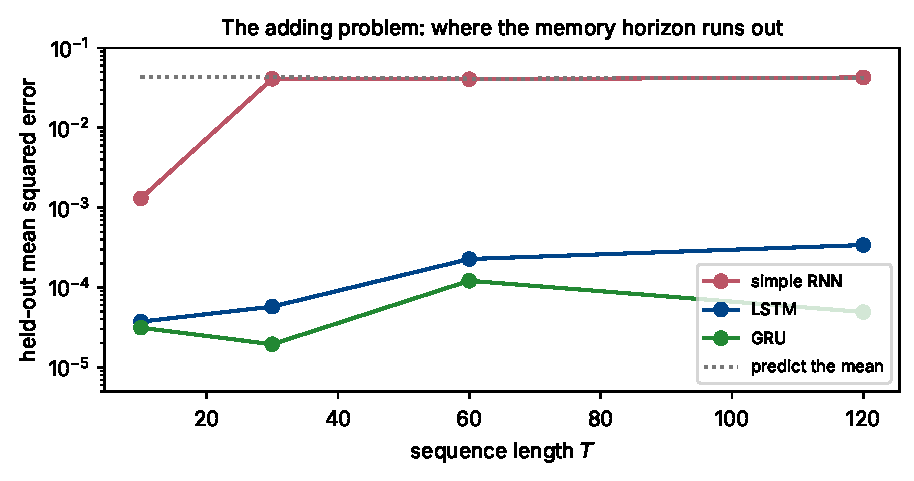
\includegraphics[width=\textwidth]{week45rnn_adding}
\end{center}
\end{column}
\begin{column}{0.5\textwidth}
\begin{lstlisting}
   T   baseline       rnn      lstm       gru
  10     0.0427    0.0013    0.0000    0.0000
  30     0.0429    0.0410    0.0001    0.0000
  60     0.0411    0.0405    0.0002    0.0001
 120     0.0425    0.0426    0.0003    0.0000
\end{lstlisting}
\small Held-out mean squared error; the baseline column is predicting the
mean.
\end{column}
\end{columns}
\begin{itemize}
  \item At $T=10$ the simple recurrent network solves the task.  At $T=30$
        it has \emph{already failed completely} -- an error equal to the
        baseline is a model that outputs the mean -- and never recovers.
  \item The LSTM and the GRU solve every case, including $T=120$, at errors
        two to three orders of magnitude below the simple RNN, with the same
        width, optimiser and epochs.  The gap between $T=10$ and $T=30$ is
        where the horizon runs out.
\end{itemize}
\end{frame}

%% =====================================================================
\begin{frame}{Exercises for the lecture (pencil and a few lines of code)}
\small
\begin{enumerate}
  \item \textbf{Linear recurrence unrolled.}  Take $\sigma_h$ linear and
        $\bm{b}=0$.  Write $\bm{h}^{(3)}$ in terms of
        $\bm{x}^{(1)},\bm{x}^{(2)},\bm{x}^{(3)},\bm{h}^{(0)}$.  Which power of
        $\bm{W}$ multiplies $\bm{U}\bm{x}^{(1)}$?  Then show that the Euler
        matrix $\bm{A}$ of Eq.~(11.15) has eigenvalues of modulus
        $\sqrt{(1-\eta\Delta t/2)^2+\Delta t^2-\eta^2\Delta t^2/4}$ to leading
        order, and evaluate it for $\eta=0$ and $\eta=0.2$ at $\Delta t=0.05$.
  \item \textbf{Two steps by hand.}  In the worked example set $w=0$.  Which of
        $\partial\mathcal{L}/\partial u$ and $\partial\mathcal{L}/\partial w$
        vanishes, and why?  Check with the five-line \texttt{torch} program.
  \item \textbf{Weighted supervision.}  In the same example give the first
        step a target $y_1=0.7$ with $\alpha_1=\alpha_2=1$ and recompute
        $\delta_1$.  Which term of the boxed recursion appears that was zero
        before?
  \item \textbf{The discrete adjoint.}  Implement Eqs.~(11.36)--(11.37) in
        NumPy or \texttt{torch} for the Euler oscillator and recover $\eta$
        from a single final position by gradient descent.  Then let
        \texttt{torch.autograd} differentiate the same Euler loop and compare.
  \item \textbf{Transient growth.}  For $\bm{W}=\bigl(\begin{smallmatrix}0.9&5\\0&0.9\end{smallmatrix}\bigr)$
        plot $\|\bm{W}^n\|_2$ against $n$ and find its maximum; repeat for an
        \texttt{nn.RNN} whose \texttt{weight\_hh} is this matrix, with
        \texttt{torch.autograd}.
  \item \textbf{Rollout.}  Train the oscillator forecaster with full BPTT and
        with chunks of length 10 (detached states); compare the one-step
        error and the free-rollout error against the horizon.
\end{enumerate}
\end{frame}

\begin{frame}{Checks on the first three exercises}
\scriptsize
\begin{enumerate}
  \item $\bm{h}^{(3)}=\bm{W}^3\bm{h}^{(0)}+\bm{W}^2\bm{U}\bm{x}^{(1)}+\bm{W}\bm{U}\bm{x}^{(2)}+\bm{U}\bm{x}^{(3)}$:
        earlier inputs pass through more applications of $\bm{W}$.  The
        exact eigenvalues of $\bm{A}$ are
        $1-\eta\Delta t/2\pm i\Delta t\sqrt{1-\eta^2/4}$, of modulus
        $1.00125$ for $\eta=0$ and $0.9962$ for $\eta=0.2$ -- the numbers of
        the integrator frame.
  \item With $w=0$: $h_2=\tanh(0)=0$, $e_2=-0.5$, $\delta_2=-0.5$, and
        $\delta_1=(1-h_1^2)\,w\,\delta_2=0$.  Hence
        $\partial\mathcal{L}/\partial u=\delta_1x_1+\delta_2x_2=0$ while
        $\partial\mathcal{L}/\partial w=\delta_2h_1=-0.5\tanh(1)=-0.380797$:
        the loss cannot teach the input weight through a zero recurrent link,
        but it can teach the link itself to open.
  \item With $\alpha_1=1$: $e_1=h_1-0.7=0.061594$, and the recursion gains
        its first term, $\delta_1=\bigl(v\,e_1+w\,\delta_2\bigr)(1-h_1^2)
        =(0.061594-0.059281)\times0.419974=0.000971$ -- the direct signal
        from the step's own output nearly cancels the one returning from the
        future.
\end{enumerate}
\end{frame}

\begin{frame}{Reading, code, and where this leads}
\footnotesize
\begin{columns}[T]
\begin{column}{0.5\textwidth}
\begin{block}{Reading}
Chapter 11 of the lecture notes, all sections -- the material of this
lecture follows it in order, including the second derivation in Section
11.3.1, the three views of BPTT in 11.4.1--11.4.7, the eigenmode discussion
in 11.5.1 and the rollout in 11.6.2.  Goodfellow et al.\ Chapter 10; Raschka
et al.\ Chapter 15; Pascanu, Mikolov and Bengio, \emph{On the difficulty of
training recurrent neural networks}, ICML 2013 (clipping, the delayed copy);
Hochreiter and Schmidhuber 1997 (LSTM); Cho et al.\ 2014 (GRU).
\end{block}
\begin{block}{Code}
Everything is in \texttt{week45rnn.ipynb}: the functions of
\texttt{make\_week45rnn\_figures.py}, Keras and PyTorch side by side, with
\texttt{mnist.npz} and \texttt{fsdd\_features.npz} next to it.
\end{block}
\end{column}
\begin{column}{0.48\textwidth}
\begin{block}{In a project}
A recurrent network is a reasonable choice when the data are sequences of
moderate length and the past matters: time series from an experiment or a
simulation, trajectories, spectra read as sequences, text.  Compare it
honestly with a dense network on the same windows and with a convolutional
network along time; report the horizon dependence of a free rollout; use
the gated cells unless the sequences are short.
\end{block}
\begin{block}{What comes after}
Attention and the transformer (Chapter 13) remove the sequential wall of
Eq.~(11.35) and the memory horizon of Corollary 11.2 at once -- by letting
every step look at every other step directly.
\end{block}
\end{column}
\end{columns}
\end{frame}

\begin{frame}{Summary}
\small
\begin{block}{What a recurrent network is}
The architecture obtained by insisting that a model respect the ordering of
its data and reuse its parameters along the time axis: a learned dynamical
system, and -- the oscillator showed, in both directions -- a learned
time-stepping scheme whose linear special case \emph{is} forward Euler.
In the libraries it is one layer, \texttt{SimpleRNN} or \texttt{nn.RNN},
fed a 3-tensor \texttt{(samples, timesteps, features)}.
\end{block}
\begin{block}{How it is trained, and why that is hard}
Backpropagation through time in three equivalent views -- the chain-rule
recursion, the pre-activation error with its outer products, the path sum
-- checked by hand on two steps and by \texttt{torch.autograd}; the Euler
case is the discrete adjoint.  The gradient across a lag is a product of
Jacobians: $10^{-18}$ over $59$ steps at $\rho(\bm{W})=0.5$, a memory
horizon of $1.4$ steps; eigenmodes, saturation and transient growth say when
to trust the bound.  Clipping handles explosion, truncation trades gradient
for memory, and a free rollout is the test that a one-step loss cannot
replace.
\end{block}
\begin{block}{What the gates change}
An additive cell path whose Jacobian is a product of forget gates: order one
over sixty steps when the gate starts open.  A simple RNN failed on
forty-step spoken digits and on the adding problem from $T=30$; the LSTM and
the GRU solved both.
\end{block}
\end{frame}

\end{document}
